\documentclass{article}
\usepackage{multicol}
\usepackage{color}
\usepackage{caption}
\usepackage{url}
\usepackage{graphicx}
\usepackage{booktabs}
\usepackage{siunitx}
\usepackage{float}
\usepackage{natbib}
\usepackage{amsmath}
\usepackage[autostyle, english = american]{csquotes}
\MakeOuterQuote{"}
\usepackage{amssymb}
\usepackage[letterpaper, total={7in, 10in}]{geometry}
\setlength{\columnsep}{0.65cm}
\setlength{\columnseprule}{1pt}
\def\columnseprulecolor{\color{blue}}
\usepackage[hidelinks]{hyperref}

\title{Towards Validity-Weighted Attenuation of Affective Noise in Student Evaluations of Teaching: An Interpretable ABSA Framework}
\author{Bassil A. A. Obeidi}

\date{April 2026}
\begin{document}
\maketitle

\begin{multicols*}{2}

\section{Introduction}
Sentiment analysis on Student Evaluations of Teaching (SET) is a popular area for the development of computational and statistical techniques to gain insights into the features of student experiences, as well as feedback for institutions and faculty. SET has historically been used as an evaluative tool to inform and guide consequential administrative decisions for academic institutions (Haskell, 1997; Simpson \& Siguaw, 2000; Irons et al., 2011). Despite this widespread usage, SET validity remains contested, with a long-running debate over the extent to which ratings reflect teaching effectiveness rather than extraneous influences (Langbein, 1994; Marsh \& Roche, 1997). Situational factors, irrelevant content, and affective noise can act as contaminants, threatening the validity of SET as a measure of instructional experience and quality (Wongsurawat, 2011; Schiekirka \& Raupach, 2015). Informal SET instruments such as RateMyProfessors.com (RMP) exhibit exacerbated contamination, due to being fully open-ended, anonymized and largely unmoderated. Thus, interpreting and acting on SET results without accounting for contamination misrepresents true teaching effectiveness and unfairly impacts faculty assessment (Haskell, 1997; Wongsurawat, 2011; Zumbach \& Funke, 2014).

As summarized by Emery et al. (2003), drawing on Dowell and Neal (1983), the systemic existence of these situational variables so thoroughly contaminates the validity of self-reported student learning and teacher effectiveness indices, that they can only be considered a measure of student satisfaction, rather than legitimate actionable feedback. 

Leveraging large-scale SET data, sentiment analysis has increasingly been used to analyze SET results, ranging from lexicon-based to deep learning and aspect-level models (Sunar \& Khalid., 2023; Bhowmik et al., 2023). Despite advances in computational SET analysis, existing research remains largely descriptive. Sentiments are extracted, patterns identified, but ratings are never intervened upon. As a result, contamination documented in the literature continues to distort the numerical ratings that institutions and students rely on. We introduce a validity-weighted attenuation framework that directly adjusts SET ratings to mitigate the influence of construct-irrelevant emotional content, while enabling inspection of the framework’s outputs and rating-adjustment process in a consequential application where important criteria cannot be fully specified (Doshi-Velez \& Kim, 2017). SET represents an ideal domain for this work: ratings are consequential, contamination is well-documented, and informal platforms like RMP (being fully anonymous and unmoderated) represent a demanding stress test for validity-aware frameworks. The present work aims to establish a foundation for future validity-aware approaches in both informal and formal SET contexts, where interpretability is essential given growing concerns about reliance on black-box systems (Rybinski \& Kopciuszewska, 2021; Zhuang et al., 2025). Findings from this research may also offer insights applicable to any open-ended feedback domain where numerical ratings are accompanied by unmoderated textual reviews.

Using RMP as a motivating case, this research explores the following research questions:\newline

\textbf{Research Questions:}

\textbf{RQ1}: How does the emotional content in pedagogical comments contribute to SET ratings?

\textbf{RQ2}: To what extent does the emotional content in pedagogically irrelevant comments contribute to SET ratings? 

\textbf{RQ3}: Can emotional attenuation of pedagogically irrelevant comments mitigate the influence of affective noise on SET ratings while preserving pedagogical signal?
\newline

To answer our research questions, we develop and apply a five-stage NLP framework to 17,121 RMP student evaluations using clause-level aspect-term categorization, fine-grained emotion extraction, pedagogical density estimation, tree-based regression modelling, and validity-weighted attenuation. Rather than excluding emotional expression, the framework proportionally down-weights content deemed irrelevant to pedagogical quality, preserving student evaluative intent while improving the signal-to-noise ratio of numerical ratings. Adjustments are auditable and grounded in textual evidence provided by the student, minimizing reliance on black-box systems where interpretability is most critical. This framework serves as a proof-of-concept, demonstrating that validity concerns in large-scale SET data can be computationally addressed in an interpretable manner.\newline

\noindent The primary contributions of this research are:
\begin{itemize}
    \item A validity-weighted attenuation framework that directly adjusts SET ratings by proportionally down-weighting construct-irrelevant emotional content. To our knowledge, the first transparent computational mechanism to operationalize CIV mitigation directly into SET rating adjustment.

    \item A theoretically grounded design bridging Messick's (1995) unified validity theory with classical reliability and robust estimation principles (Cronbach, 1951; Huber, 1964), translating established psychometric justifications into a concrete computational mechanism and laying groundwork for future validity-aware frameworks.

    \item An interpretable and auditable adjustment mechanism, ensuring each rating adjustment is directly traceable to specific topic-level emotions and pedagogical content density. 
\end{itemize}

The subsequent sections are structured as follows: Section 2 delves into the literature review of our research, providing the evidence in the literature of SET contamination and validity concerns, an overview of recent research related to computational SET analysis and textual quality quantification, and finally a psychometric, statistical, and explainability-grounded justification for the proposed attenuation mechanism. Section 3 presents an exploratory data analysis of the RMP dataset and outlines our methodology, including the full framework pseudocode and worked end-to-end examples illustrating the framework's attenuation behaviour across distinct review types. Section 4 covers framework validation. The results are presented in Section 5, followed by the discussion in Section 6. Limitations and future work are in Sections 7 and 8, respectively, with the conclusion in Section 9. 

\section{Literature Review}
\subsection{SET Contamination}
Previous research in educational psychology has documented emotional and affective noise in SET. The following subsection reviews key findings from the literature to establish that SET validity depends on the content an instrument elicits, and that situational factors and pedagogically irrelevant content act as a measurable contaminant and source of noise in SET data.

Marsh and Roche (1997) scrutinize the validity, bias and utility of SET in a comprehensive review. They conclude that under appropriate conditions, SET are multidimensional, reliable, and relatively valid against a variety of indicators of effective teaching. However, they condition this validity on the content and the coverage of the evaluation items, indicating that ``scores averaged across an ill-defined assortment of items offer no basis for knowing what is being measured'' (p. 1187). Validity is therefore treated as a property of the content an instrument elicits rather than of the instrument itself. Under this criterion, unconstrained and open-ended instruments offer no design guarantee on the composition of the content they collect.

Wongsurawat (2011) analyzes the value of open-ended SET feedback and proposes a conceptual framework of comments. The author suggests that some students do not put sufficient thought and effort into evaluating their instructors. Importantly, white noise, or pedagogically irrelevant content, is identified as a source of measurement error in SET instruments. A conceptual four-quadrant framework comparing the correlation of subjective and objective comments to class averages is proposed to judge the reliability and representativeness of SET feedback. Wongsurawat indicates that comments that have little to no correlation with average evaluations should be discounted, and that administrators would benefit from metrics quantifying comment quality and reliability.

Schiekirka and Raupach (2015) systematically review which factors influence student ratings in medical education course evaluations in order to improve future education evaluation tools. They indicate that situational factors such as student characteristics, performance level and evaluation process might act as confounders, thus threatening the validity of evaluation results. They advocate for administrative awareness on the variety of factors that influence student ratings and encourage additional research into the control of potential confounders and development of robust evaluative instruments.

Li et al. (2025) conduct a qualitative study using semi-structured interviews with medical students. Thematic analysis reveals that emotional interactions between teachers and students may lead students to overlook the actual quality of teaching. They suggest that teaching evaluations are not only feedback directed to pedagogical experiences, but also reflections of students’ emotional, affective and relational states.

The aforementioned studies identify and measure affective noise as both a systematic and consequential source of measurement error in SET. However, these studies rely mainly on surveys and experiments without leveraging large-scale textual data for quantification and error attenuation. This gap underscores the need for computational methods that extract topic-specific emotional signals to mitigate the influence of affective noise on SET ratings.

\subsection{Computational SET Analysis}
Sentiment analysis in the educational domain has garnered considerable attention in recent years (Dalipi et al., 2021). However, computational analysis of SET results has been a focus of research since at least 2011. This subsection aims to provide a methodological introduction to the application of computational techniques in the SET domain.

Kechaou et al. (2011) train a supervised learning model on 2000 e-learning reviews and use the model to predict the overall sentiment of reviews. Their results demonstrated that sentiment polarity can be extracted from educational reviews with reasonable accuracy (F1 = 0.803).

Rajput et al. (2016) supplement Likert-scale questions with lexicon-based sentiment analysis on SET reviews, finding a strong correlation (R = 0.64) between sentiment scores and likert-scale ratings. Per-class evaluation of their sentiment classifier shows strong performance on positive sentiments (F1 = 0.95) but lower on negative (0.67) and mixed sentiments (0.57).

Iatrellis et al. (2024) use VADER (Valence Aware Dictionary and sEntiment Reasoner) to compute compound sentiment scores for a multi-institutional dataset of 1,151 student reviews. By aggregating these scores at the advisor level, they report a significant positive correlation ($r^2 = 0.561$) between sentiment analysis results and mean Likert ratings per advisor.

An approach by Mihai (2024) uses VADER to determine sentiment polarity within SET reviews. Mihai concludes that VADER can be used for quick and minimal sentiment analysis but struggles with contextual and nuanced emotional expressions in SET reviews.
 
Prior research demonstrates that simple sentiment analysis on SET reviews can reliably extract coarse sentiments that have moderate-to-strong correlation with numerical ratings. However, these early approaches combine sentiments as a single aggregate, limiting their ability to capture complex emotional context and signals, and act as inputs for validity-weighted frameworks. These limitations provide motivation for more advanced approaches that utilize deep learning and aspect-based sentiment analysis (ABSA) to analyze SET results.

Transformers-based deep learning models represent the next technological leap in Natural Language Processing (NLP) for sentiment analysis. Transformers-based models, such as fine-tuned BERT (Bidirectional Encoder Representations from Transformers) variants, enable analysis across an emotional spectrum.

Rybinski and Kopciuszewska (2021) modify and fine-tune BERT to predict a numerical rating or topic from fine-grained student review sentiments, achieving a validation accuracy of 84\%. However, they note that deep learning NLP models can unintentionally amplify emotional biases and raise concerns about interpretability issues in black-box models.

Shuqin and Raga (2024) combine the contextual strengths of BERT with the sequence modelling of BiLSTM (Bidirectional Long Short-Term Memory) for fine-grained sentiment analysis of student evaluations. This hybrid approach achieves $F1 > 0.96$ after data cleaning. 

Although deep learning approaches provide a finer-grained representation of emotional signals contained within SET reviews, analyzing sentiment per review aggregates multiple review aspects within a single numerical rating, in which affective noise is introduced to different extents. Therefore, a validity-weighted attenuation framework likely requires finer-grained representation of sentiments. 

ABSA offers the next computational advancement in sentiment analysis techniques in the SET domain. There exists a multitude of similar studies performing ABSA on SET reviews reporting promising findings on ABSA utility and performance (Bhowmik et al., 2023; Nikolic et al., 2020; Jazuli et al., 2025).

Ren et al. (2022) employ ABSA using a combination of deep learning and dictionary-based approaches to automatically calculate the emotional orientation of SET reviews. Student reviews are computationally separated into references to distinct teaching topics, and sentiment analysis is used to determine the sentiments associated with each topic. This method results in a precision, recall, and F1 score of 0.80, 0.79 and 0.79, respectively.

In the progression from early lexicon-based studies, deep learning emotional spectra, to recent finer-grained ABSA techniques, sentiments are extracted reliably. Yet, previous studies focus on extraction and prediction, without introducing mechanisms to reduce the influence of affective noise. This gap has motivated the progression to transparent validity-aware frameworks that prioritize interpretability over reliance on black-box systems.

\subsection{Computational Validity Analysis of SET}
The following subsection examines how recent research uses computational techniques to quantify and analyze situational biases and pedagogical relevance in large-scale datasets.

Kopciuszewska and Rybinski (2024) quantify cumulative SET bias using regression models to determine if biases vary across levels of SET scores and time. Their analysis demonstrates that systematic bias exists in SET reviews and can significantly distort ratings, intensified during the shift to E-learning during the COVID-19 pandemic. Additionally, they propose the use of adjusted SET scores to provide a more accurate reflection of teaching performance. 

Kim et al. (2025) study the sentiments in SET reviews directed towards six distinct teaching topics and make use of Bayesian ordinal regression to identify drivers of SET scores. Their findings suggest that students’ SET ratings are primarily correlated with the personal characteristics of the lecturer, over teaching dimensions.

While these studies quantify the existence of situational biases that contaminate the validity of SET results, they do not provide a framework for attenuating the influence of affective noise on numerical scores. 

Past research has also examined ways to computationally estimate pedagogical relevance or quality of student comments. 

Sorour et al. (2015) employ latent semantic analysis and clustering to predict student grades from lesson reflections. They used the PCN method which categorizes comments into previous (P), current (C), next (N), and other (O) activities. Isolating current pedagogically relevant comments and filtering out semantically distant or noisy comments resulted in an improvement of prediction accuracy from 66.4\% in the baseline model to 86.4\% when using a combined similarity and overlap measuring method on cleaned data.

Similar work in computational linguistics and educational text analysis (Louis \& Nenkova, 2013; Xiong \& Litman, 2011) develop models to quantify the utility and quality of textual feedback. Their results suggest that not all comments in student evaluative texts carry equal pedagogical value and relevance. However, more work is needed to implement these detection systems to mitigate the impact of affective noise on SET.

\subsection{Psychometric Validity \& Explainable Intervention}
Messick (1995) identifies two primary threats to validity in assessment systems: construct underrepresentation and construct-irrelevant variance (CIV). Construct underrepresentation occurs when an assessment fails to adequately capture the dimensions of the construct it is intended to measure. Messick does not address student feedback systems by name; however, his unified theory explicitly extends to any assessment in which observed behaviors or responses are coded or summarized into scores, a formulation that directly encompasses SET. These validity threats are particularly pronounced when collected using informal and anonymous devices such as RMP.

Addressing validity concerns within SET does not require excluding low-utility reviews. Classical reliability theory holds that measurement quality improves by reducing error variance rather than excluding observations (Cronbach, 1951). Robust estimation theory formalizes this principle, showing that down-weighting high-noise observations produces more stable and less biased estimates than exclusionary approaches (Huber, 1964). Within the SET domain, Marsh and Roche (1997) advocate for a conservative approach for bias mitigation, arguing that corrections should account for known sources of contamination while preserving students' overall evaluative intent. They further caution that corrections applied without regard to valid variance risk ``throwing the validity baby out with the bias bathwater'' (p. 1197), removing genuine signal alongside the contaminant. This supports a bounded, content-targeted adjustment rather than a global correction.

Recent psychometric work has demonstrated that CIV can be identified and mitigated in constructed-response assessments. Zhai et al. (2021) propose a Many-Facet Rasch Measurement framework that identifies three sources of CIV: the variability of assessment item scenarios, judging severity, and rater scoring sensitivity to the scenarios in tasks. Their framework mitigates these sources of CIV when estimating examinee ability. However, their approach operates under controlled conditions including expert-defined rubrics, trained raters, and a shared observable stimulus (a common video) against which responses can be evaluated. These conditions do not extend to large-scale SET systems.

Because pedagogical experience cannot be feasibly observed at the scale of SET data, adjustments to SET scores cannot
be validated against an objective ground truth. In this setting, interpretability can help make the effects of
modelling assumptions and the framework's adjustment process visible for scrutiny (Doshi-Velez \& Kim, 2017).

\subsection{Domain-Adjacent Applications}
The previous computational sections have primarily focused on sentiment analysis within SET. Similar techniques have been increasingly applied across other open-ended feedback domains. 

ABSA is used to extract fine-grained topic-specific sentiments in consumer feedback systems such as online product and user-experience reviews, in the healthcare sector examining patient feedback and hospital reviews and in the professional sector for HR survey responses (Ballas et al., 2024; Skorin \& Petrenko, 2025; Nguyen, 2025; Alkhnbashi et al., 2024; Lee \& Song, 2024; Dina \& Juniarta, 2020; Rink et al., 2024).

There are recent examples of research that incorporates these signals into mechanisms that reduce the impact of CIV on numerical ratings. Online product or service ratings can be adjusted by controlling for the impact of suspicious review patterns or biased reviewer tendencies (Pelaez et al., 2026; Lim \& Tucker, 2017). In the professional domain, validity-aware ratings can be generated by applying a regression vector stochastic gradient descent classifier to staff satisfaction surveys (Gaye et al., 2021).

These examples demonstrate the potential for transparent validity-weighted attenuation frameworks to be adapted across numerous open-ended feedback domains.

\subsection{Research Gap}
Existing literature shows that CIV and other sources of noise systematically contaminate SET, influencing numerical ratings in ways unrelated to actual pedagogical experience. Advances in NLP demonstrate that topic-specific emotional sentiment in SET reviews can be reliably extracted. Recent large-scale studies confirm that CIV manifests in real-world evaluation data substantially distorting SET ratings. Reliability and robust estimation theory therefore support the use of proportional down-weighting to reduce the influence of CIV, provided that construct-relevance can be estimated. Since there is no objective ground truth to validate adjusted scores, frameworks that attenuate CIV must treat interpretability and transparency as essential design constraints.

Despite computational advances in SET analysis, existing studies remain largely descriptive. To the best of our knowledge, no prior work provides a transparent computational framework that leverages topic-level sentiment to identify and attenuate construct-irrelevant emotional content and mitigate the impact of CIV on SET ratings.

We address this gap by introducing an interpretable ABSA framework combining clause-level aspect-term categorization, fine-grained emotion extraction, pedagogical density estimation, tree-based regression modelling, and validity-weighted attenuation. This framework estimates the contribution of pedagogical signal and affective noise to numerical ratings (RQ1, RQ2), and generates validity-weighted attenuated scores reflecting reduced influence of construct-irrelevant emotional content (RQ3). The proposed framework combines fine-grained NLP sentiment modelling with psychometric theories of validity and statistical approaches for measurement error reduction.
\section{Methodology}
\subsection{Data}
As a source of data, we choose SET reviews from RMP because it is a popular professor and course review website offering anonymous use by any student. Additionally, being an informal SET system, it represents a stress test for our framework's capacity to mitigate CIV. RMP lists a strict "no scraping" policy, and despite attempts to contact site administrators to request permission to source data directly from the site, no permission was granted. Instead, we use an open-source dataset provided by He (2020), sourced from RMP. This dataset comprises more than 19,000 individual SET reviews directed towards hundreds of professors. These SET reviews consist of a textual section, numerical rating (1-5) and various meta-tags used on RMP to classify different teaching styles and qualities. The dataset also included demographic information measured by the original researchers. For our purposes, the meta-tags and demographic information is not used.

Table~\ref{tab:dataexamples} presents three representative reviews from the dataset, 
illustrating the informal and varied nature of RMP student feedback. Reviews range from 
concise evaluations to multi-sentence reflections spanning several 
pedagogical dimensions, and frequently contain informal language, punctuation 
irregularities, and non-pedagogical commentary.

\begin{table*}[ht]
    \caption{Data examples from the RMP dataset.}
    \centering
    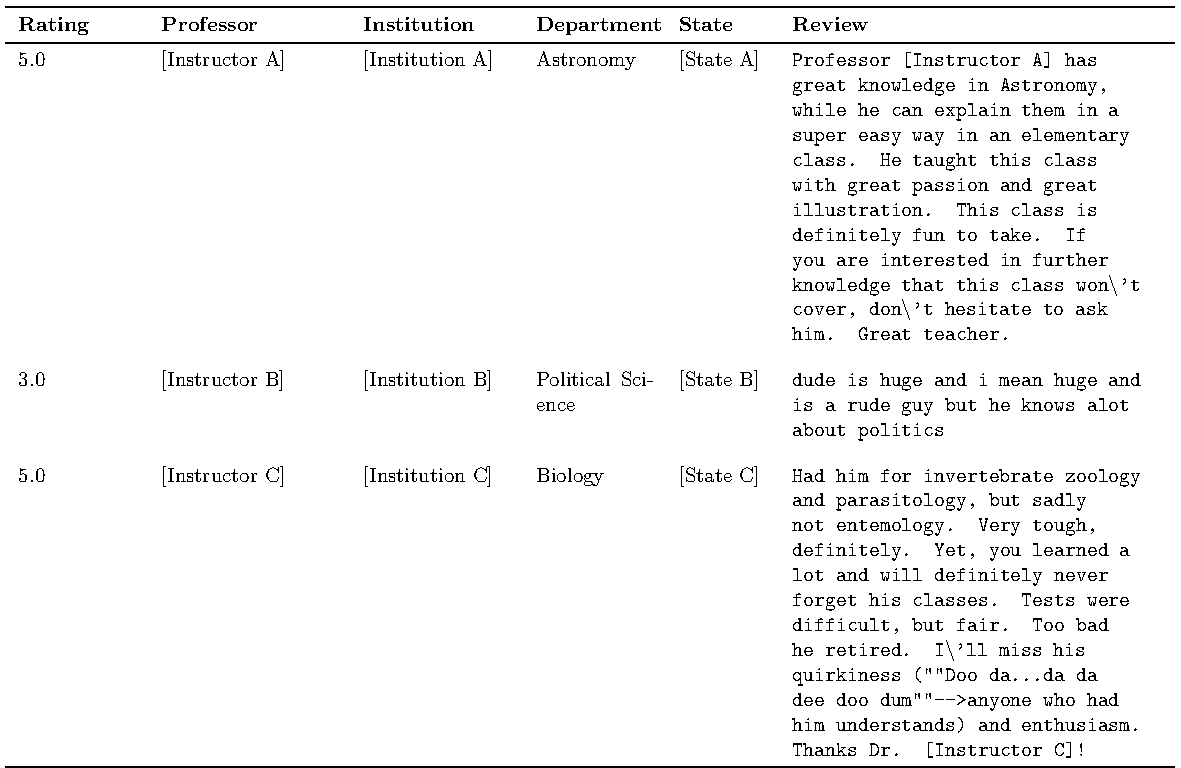
\includegraphics[width=\linewidth]{Diagrams/pdfs/exampledata.pdf}
    \label{tab:dataexamples}
\end{table*}

\subsection{Data Preprocessing}
Performing ABSA on SET reviews from RMP is a difficult task. Reviews can be written in multiple languages and contain informal language, spelling, grammatical and punctuation errors, censored profanity, UTF encoding errors (such as mojibake), and other hindrances to NLP models. Additionally, RMP has a built-in profanity censoring feature that infrequently incorrectly censors words or substrings within words. We excluded all non-English reviews as the NLP models used only support English input. Furthermore, any reviews that contained the RMP automatic censorship string "****" are also excluded as its application was prone to error. Finally, reviews in which the professor being reviewed has fewer than 8 total reviews across the dataset are excluded. After these exclusions, the total number of reviews in the dataset is reduced to 17,121. 

Preprocessing this informal text is critical for the accuracy of later ABSA stage. Several different strategies are used to clean the text. First, encoding errors or mojibake are fixed using a combination of Python library ftfy (fixes text for you), regular expressions, and string normalization using NFKD (Normalization Form Compatibility Decomposition). Next, text is standardized to lowercase, and abbreviations and titles are expanded. This step is particularly critical, as periods used in abbreviations or titles can cause unwanted clause segmentation.\newline

\textbf{Examples}:

\begin{itemize}
    \item \verb|"Mr. [Instructor] is a great teacher."| $\rightarrow$ \verb|"mr [instructor] is a great teacher."|
    \item \verb|"BEST PROF. EVER!"| $\rightarrow$ \verb|"best professor ever!"|
    \item \verb|"t.a."| $\rightarrow$ \verb|"ta"|
    \item \verb|"e.g."| $\rightarrow$ \verb|"eg"|
\end{itemize}

We replace informal language with equivalent formal representation using regular expressions.\newline

\textbf{Examples}: 

\begin{itemize}
    \item \verb|"ta"| $\rightarrow$ \verb|"teaching assistant"|
    \item \verb|"t/f"| $\rightarrow$ \verb|"true or false"|
    \item \verb|"mt"| $\rightarrow$ \verb|"midterm"|
    \item \verb|"hw"|, \verb|"hwk"|, \verb|"hmwk"| $\rightarrow$ \verb|"homework"|
\end{itemize}

Character emojis and self-censored profanity are replaced with textual tags.\newline

\textbf{Examples}:

\begin{itemize}
    \item \verb|"!$#?"| $\rightarrow$ \verb|"profanity"|
    \item \verb|":^)"| $\rightarrow$ \verb|"emoji"|
    \item \verb|"d(^_^o)"| $\rightarrow$ \verb|"emoji"|
\end{itemize}
    
Punctuation and whitespace are cleaned.\newline

\textbf{Examples}

\begin{itemize}
    \item \verb|"~~~my god!~"| $\rightarrow$ \verb|"my god!"|
    \item \verb|"------pros: 1)"| $\rightarrow$ \verb|"pros 1"|
    \item \verb|"pass.she"| $\rightarrow$ \verb|"pass. she"|
\end{itemize}

After these changes, the text is significantly cleaner. Further processing could be applied such as spell-checking, stemming and lemmatization, however, it would likely result in a loss of contextual information for future steps in the framework.

\subsubsection{Exploratory Data Analysis}
The following descriptive analyses characterize the preprocessed dataset of 17,121 reviews used throughout this research, following the exclusion criteria described above.

Figure~\ref{fig:rating_freq} shows the distribution of numerical ratings across the dataset. The distribution is negatively skewed, with 5-star reviews constituting the largest proportion of the dataset. This skew has implications for downstream regression modelling and attenuation outcomes.

\begin{figure}[H]  
    \centering
    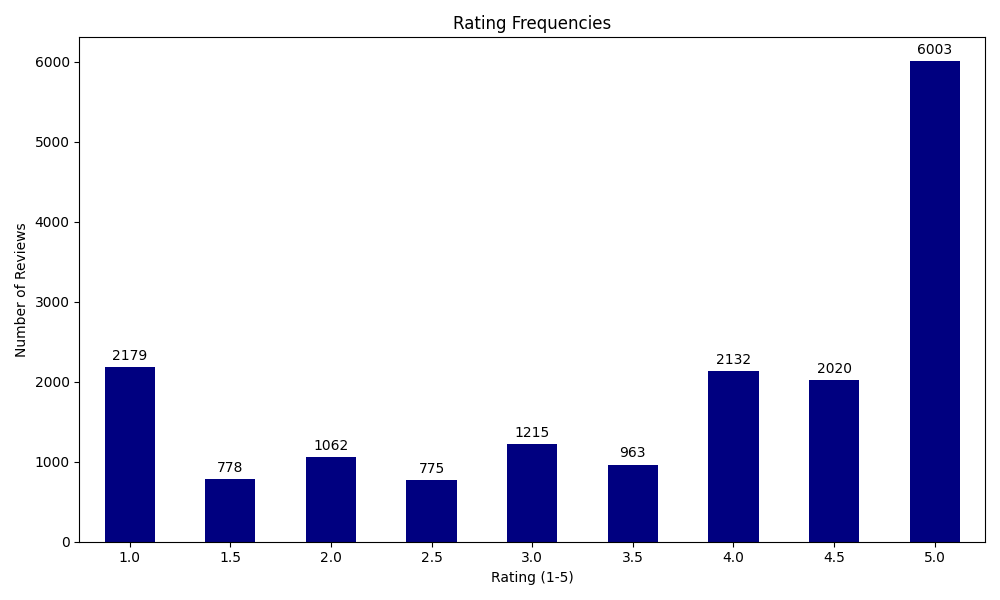
\includegraphics[width=\columnwidth]{Diagrams/Data Analysis/ratingfreq.png}
    \caption{Rating frequencies.}
    \label{fig:rating_freq}
\end{figure}

Figure~\ref{fig:revlengthdist} presents the distribution of review text length measured in word count. Review lengths follow a right-skewed distribution with a mean of 40.1 words and a standard deviation of 20.3, reflecting the open-ended and unstructured 
nature of RMP reviews. The majority of reviews are relatively concise, though a long tail of more elaborate reviews is observed.

Figure~\ref{fig:profreviewdist} presents the distribution of review counts per professor. The distribution exhibits a plateau across 8 to approximately 16 reviews, before concentrating sharply around 20 reviews.

\begin{figure*}[btp]  
    \centering
    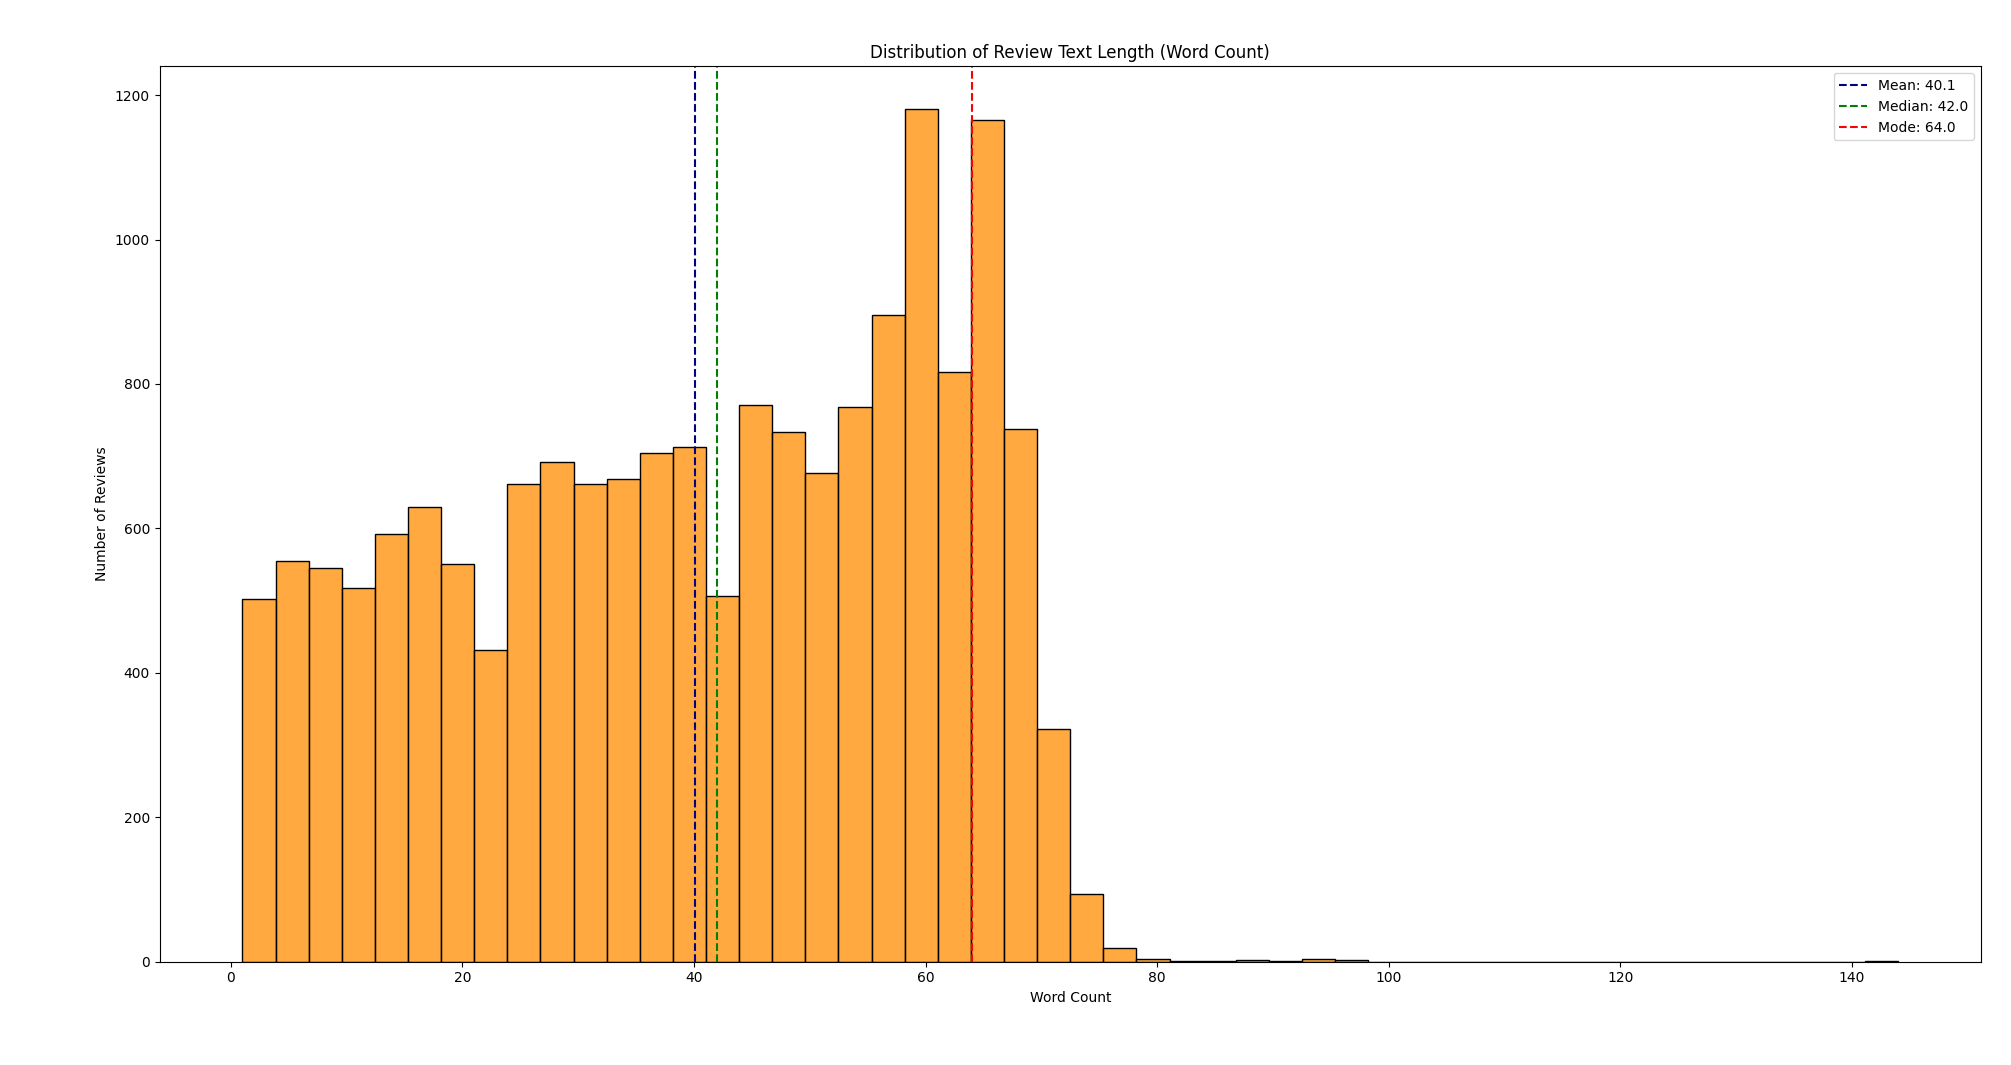
\includegraphics[width=\linewidth]{Diagrams/Data Analysis/reviewlengthdistribution.png}
    \caption{Distribution of review lengths (word-count).}
    \label{fig:revlengthdist}
\end{figure*}

\begin{figure*}[btp]  
    \centering
    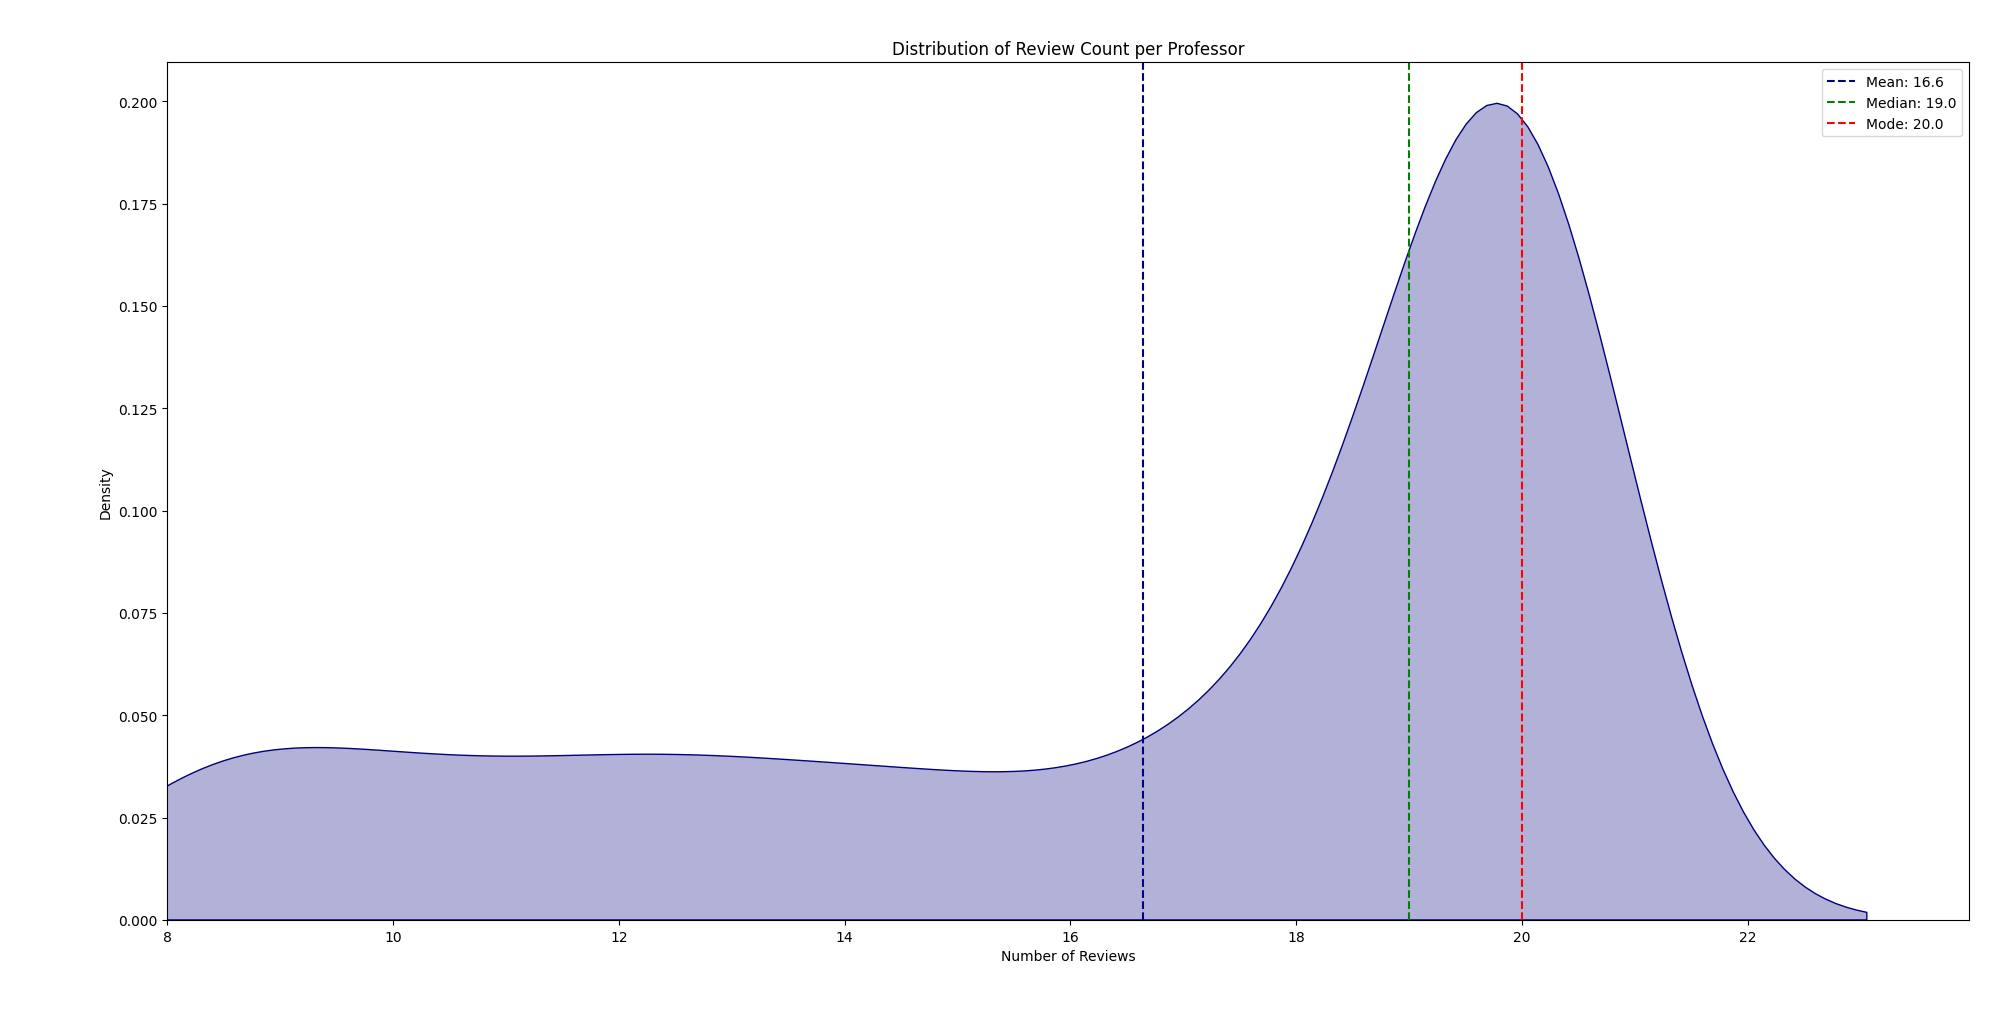
\includegraphics[width=\linewidth]{Diagrams/Data Analysis/profreviewcountdistribution.png}
    \caption{Distribution of review counts per professor.}
    \label{fig:profreviewdist}
\end{figure*}

\subsection{Model Pipeline}
The framework processes each review through a five-stage pipeline. It extracts clause-level emotions across pedagogical and non-pedagogical topics and computes a pedagogical density metric. This density metric is used to proportionally down-weight construct-irrelevant sentiment while preserving pedagogically relevant signals. An overview of the methodology can be described as follows:

\textbf{1. Clause Extraction and Categorization}

Reviews are separated into individual clauses using \texttt{spaCy}. Individual clauses are categorized into distinct pedagogical topics using a Sentence-BERT style embedding model and cosine similarity comparisons. If a statement falls below a certain threshold, it is not classified as related to pedagogy and instead is categorized as \textit{Miscellaneous}.

\textbf{2. Pedagogical Density Calculations}

A pedagogical density metric is calculated for each review, representing the relative occurrence of pedagogical feedback in the overall review.

\textbf{3. Aspect-Based Sentiment Analysis}

These separated and categorized clauses are fed into \texttt{SamLowe/roberta-base-go\_emotions}, a deep learning sentiment analysis model based on RoBERTa, trained on the \texttt{go\_emotions} dataset, in order to determine emotional sentiment within reviews.

\textbf{4. Tree-Based Regression Modelling}

Numerical ratings are modelled as a function of their associated topic sentiment features, using CatBoost (tree-based) regression. This step reveals how sentiment directed to each categorization topic contributes to the numerical ratings across the entire dataset.

\textbf{5. Validity-Weighted Attenuation and Rating Adjustment}

\textit{Miscellaneous} sentiment is down-weighted using pedagogical density, to mitigate the influence of pedagogically irrelevant polarized emotions. Finally, using the previously trained CatBoost model, adjusted ratings are generated by adding the difference between attenuated and baseline predicted ratings from raw student ratings.

\begin{figure*}[btp]  
    \centering
    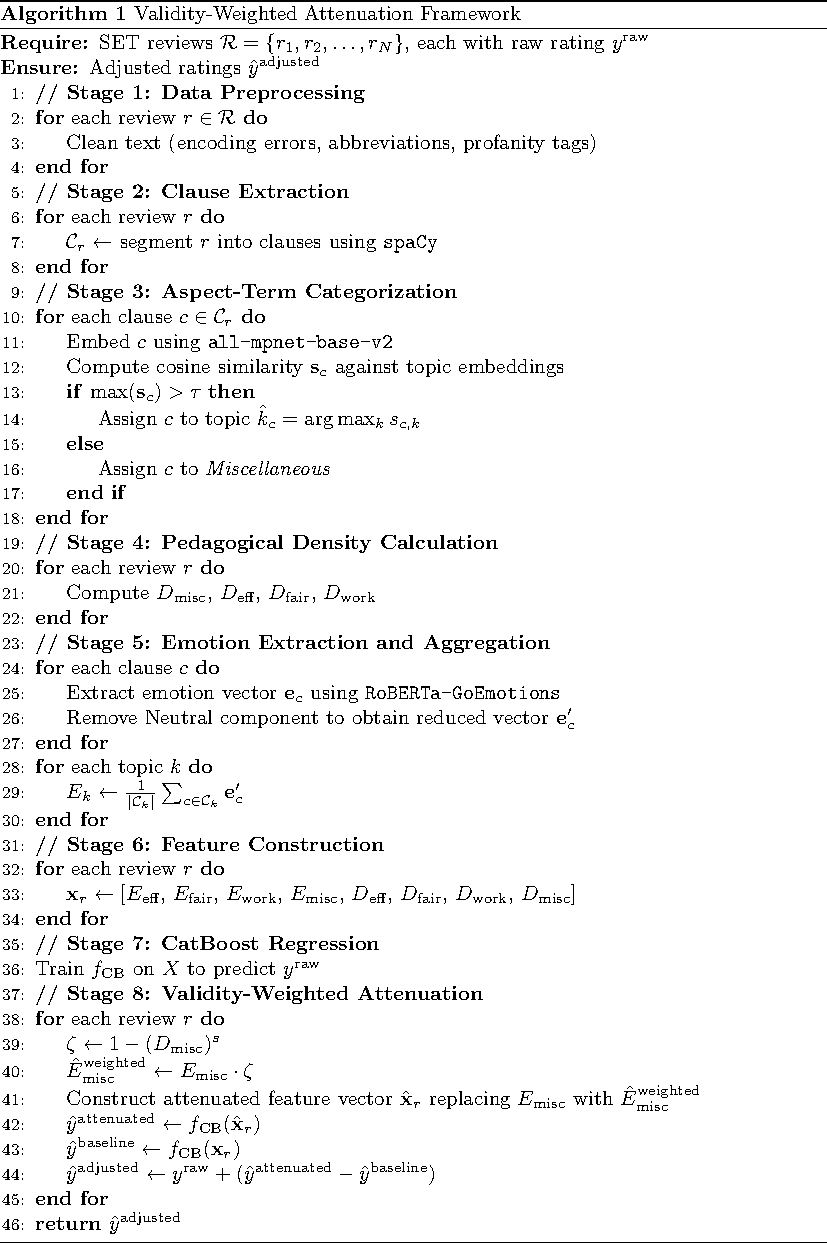
\includegraphics[trim=0 0 45 0, clip, width=0.83\linewidth]{Diagrams/pdfs/pseudocode.pdf}
    \caption{Pseudocode for the framework.}
    \label{fig:pseudocode}
\end{figure*}

Pseudocode outlining our methodology is presented in Figure~\ref{fig:pseudocode} and a schematic diagram of our framework is shown in Figure~\ref{fig:overall-schematic}.  

\begin{figure*}[btp]  
    \centering
    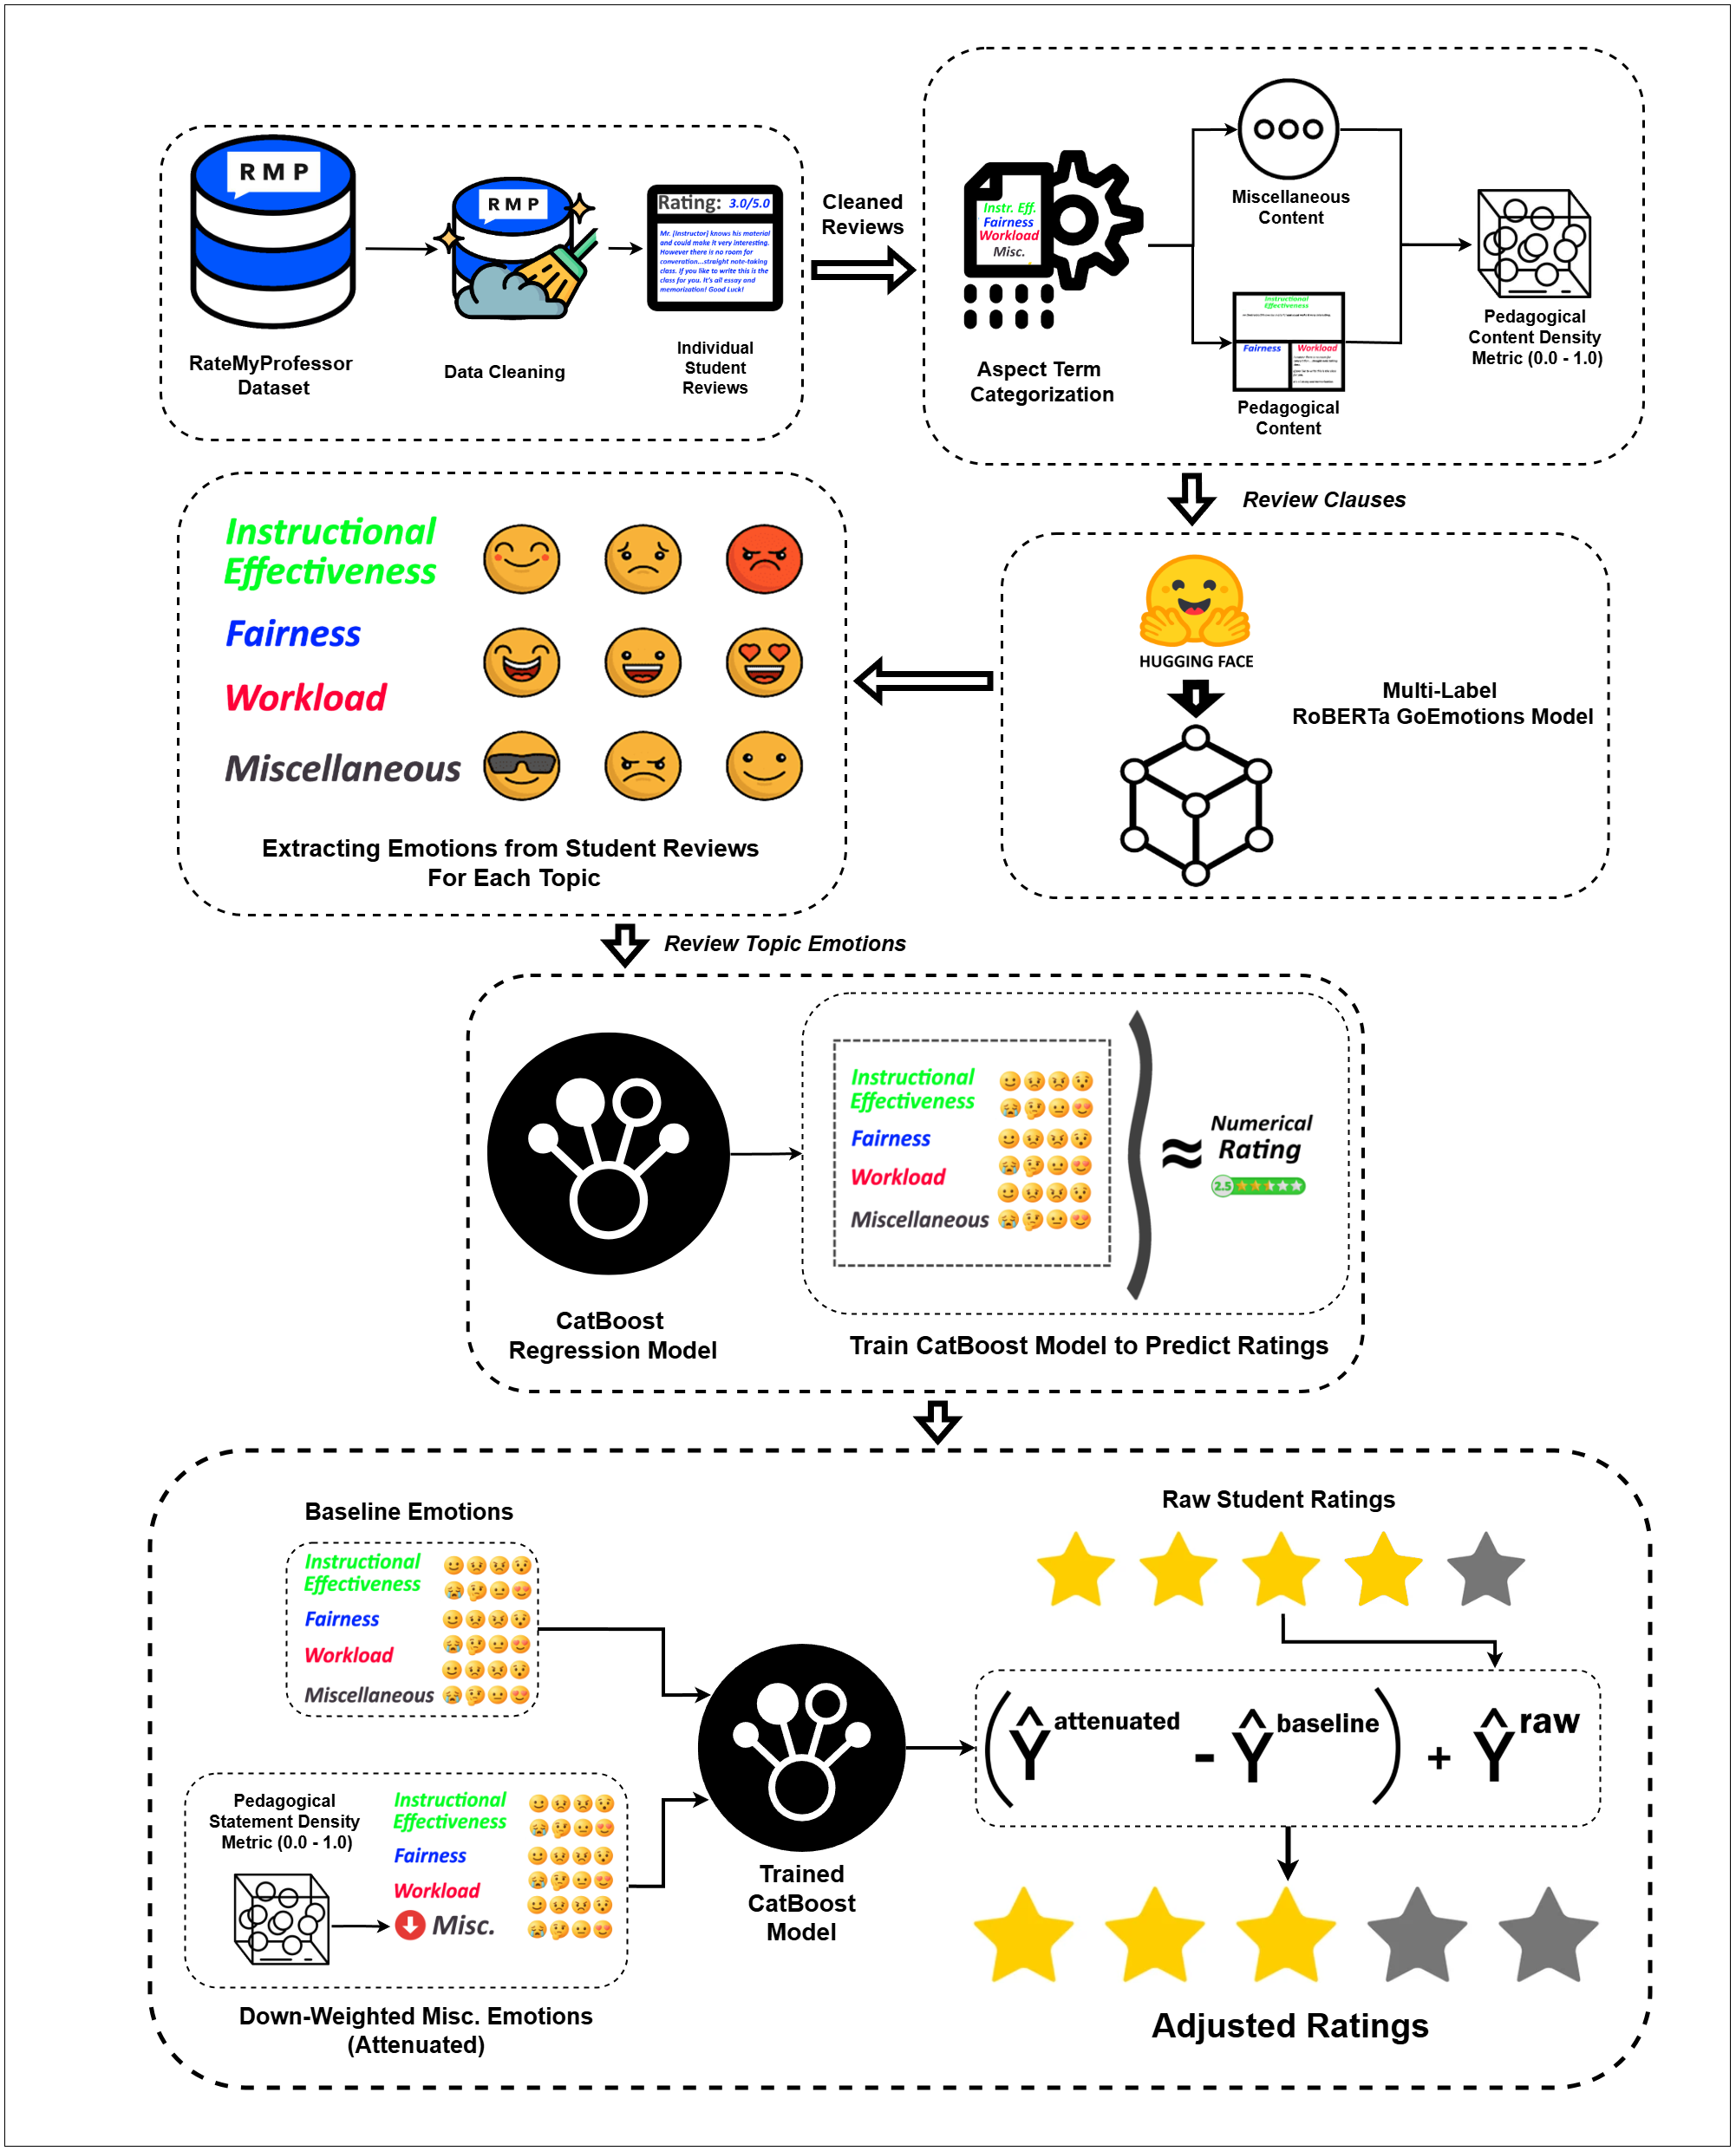
\includegraphics[width=\linewidth]{Diagrams/Schematic_Diagrams/FinalSchematic.png}
    \caption{Schematic diagram of our framework.}
    \label{fig:overall-schematic}
\end{figure*}
\subsection{Clause Extraction}
Cleaned text is separated into individual clauses using \texttt{spaCy}'s \texttt{en\_core\_web\_sm} model which segments text based on punctuation while attempting to avoid splits on non-statement punctuation.
Two additional rules supplement \texttt{spaCy} when punctuation is sparse: splitting on commas and stop-words (but, so, yet) when no sentence-ending punctuation exists, or using aggressive stop-word separation for reviews with no punctuation.\newline

\textbf{Example 1. (\texttt{spaCy} sentence segmentation)}\newline

\textit{Overall Review}:

"had him for invertebrate zoology and parasitology, but sadly not entemology. very tough, definitely. yet, you learned a lot and will definitely never forget his classes. tests were difficult, but fair. too bad he retired. i'll miss his quirkiness doo da... da da dee doo dum anyone who had him understands and enthusiasm. thanks doctor [instructor]!"\newline

\textit{Clause 1}:
"had him for invertebrate zoology and parasitology, but sadly not entemology."

\textit{Clause 2}:
"very tough, definitely."

\textit{Clause 3}:
"yet, you learned a lot and will definitely never forget his classes."

\textit{Clause 4}:
"tests were difficult, but fair."

\textit{Clause 5}:
"too bad he retired."

\textit{Clause 6}:
"i'll miss his quirkiness doo da..."

\textit{Clause 7}:
"da da dee doo dum anyone who had him understands and enthusiasm."

\textit{Clause 8}:
thanks doctor [instructor]!\newline

\subsection{Aspect-Term Categorization}

The next stage in the processing pipeline assigns each review clause to one of three pedagogically relevant categories (\textit{Instructional Effectiveness}, \textit{Fairness \& Grading}, and \textit{Workload \& Difficulty}) or to a \textit{Miscellaneous} category. This task is formulated as an \emph{aspect-term categorization} (ATC) problem, also referred to in the literature as \emph{aspect topic detection} or \emph{aspect topic classification}.

Semantic representations of each pedagogical topic are constructed by encoding concise textual descriptions of the categories using a pretrained sentence-embedding model (\texttt{all-mpnet-base-v2}). The resulting sentence embeddings serve as dense vector representations for each topic. Review clauses are embedded using the same model.

Each pedagogical topic is defined using multiple short natural-language descriptions of common student expressions. For example, the
\textit{Instructional Effectiveness} topic includes descriptions such as "clear and effective explanations of concepts" and "lectures are well-organized and easy to follow", while \textit{Fairness \& Grading} captures language related to grading, equitable treatment, leniency, and evaluation policies. \textit{Workload \& Difficulty} captures references to assignment volume, exam difficulty, and time demands.

\begin{figure*}[t]
    \centering
    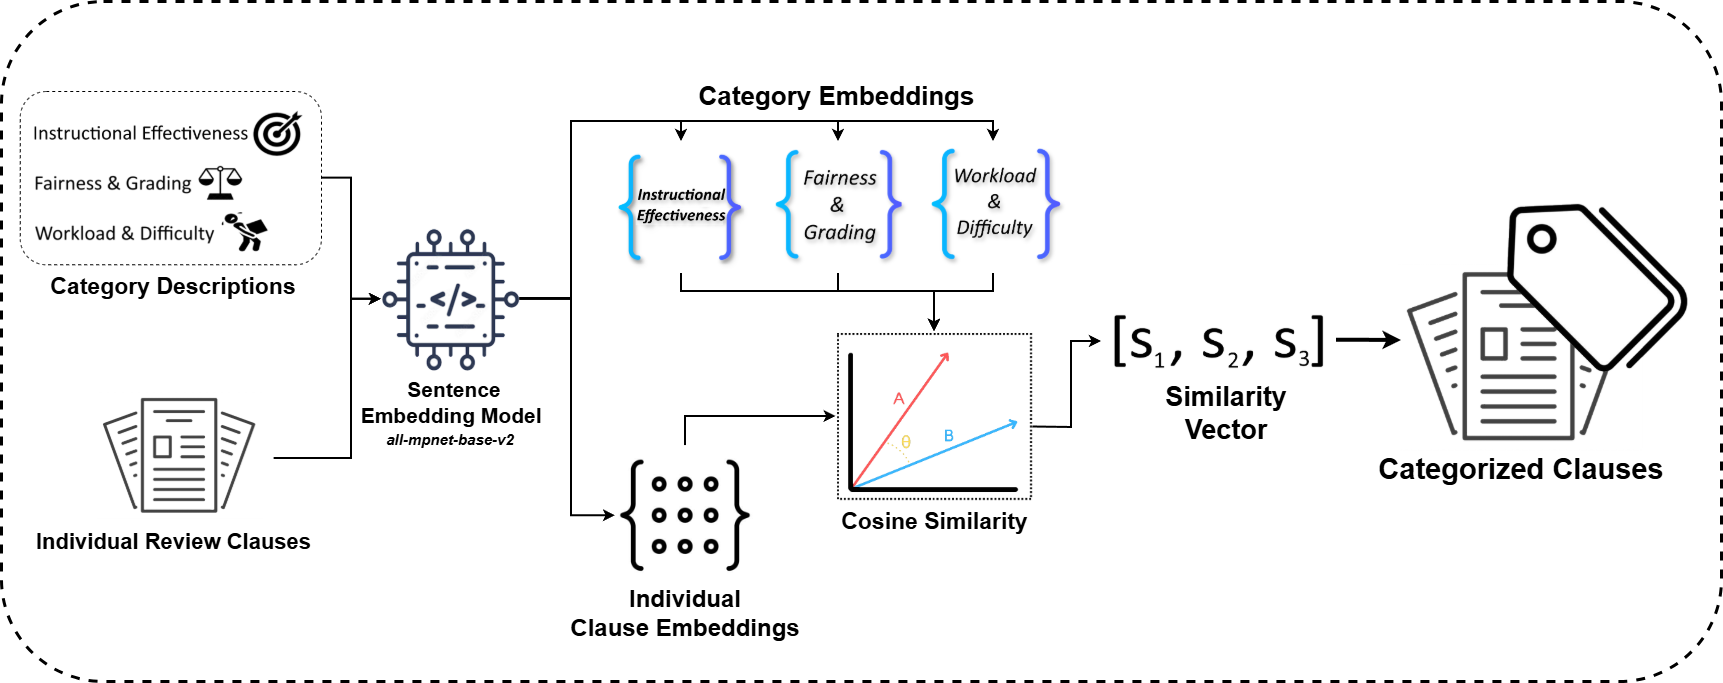
\includegraphics[width=\textwidth]{Diagrams/Schematic_Diagrams/atc-schematic.png}
    \caption{Schematic diagram of the aspect-term categorization stage.}
    \label{fig:atc_overview}
\end{figure*}

Clause–topic similarity is computed using cosine similarity between the clause embedding and each topic embedding, producing a similarity vector
\begin{equation}
\mathbf{s}_c = \big( s_{c,\text{eff}},\, s_{c,\text{fair}},\, s_{c,\text{work}} \big),
\end{equation}
where each component represents the semantic similarity between clause $c$ and a pedagogical topic.

Each clause is first assigned a candidate topic by identifying the highest-scoring pedagogical category:
\begin{equation}
\hat{k}_c = \arg\max_{k \in \{\text{eff},\,\text{fair},\,\text{work}\}} s_{c,k}
\end{equation}

The candidate topic is accepted only if its similarity score exceeds a predefined threshold $\tau$; otherwise the clause is categorized as \textit{Miscellaneous}:
\begin{equation}
\text{topic}(c) =
\begin{cases}
\hat{k}_c, & \text{if } s_{c,\hat{k}_c} > \tau, \\
\textit{Miscellaneous}, & \text{otherwise}.
\end{cases}
\end{equation}

where $\tau = 0.25$. This threshold was selected through validation on a development subset of manually inspected clauses, balancing precision and coverage.\newline


\textbf{Example 1. (ATC)}

\textit{Clause:}

"yet, you learned a lot and will definitely never forget his classes."

\textit{Similarity Vector:} $[0.39,,0.25,,0.31]$

$\max(\mathbf{s}_c) = 0.39 > 0.25$, the clause is categorized as \textit{Instructional Effectiveness}.\newline

\textbf{Example 2. (ATC)}

\textit{Clause:}

"i'll miss his quirkiness doo da..."

\textit{Similarity Vector:} $[-0.03,,0.00,,-0.03]$

$\max(\mathbf{s}_c) = 0.00 < 0.25$, the clause is categorized as \textit{Miscellaneous}.\newline

\texttt{all-mpnet-base-v2} was selected for ATC as it provides strong semantic generalization without requiring labelled training data. By encoding both clause text and category descriptions as dense semantic vectors, the model captures meaning across diverse phrasings and informal language common within RMP reviews. 

A schematic overview of the ATC model is provided in Figure~\ref{fig:atc_overview} and validation metrics are provided in Section~4.1.

\subsection{Pedagogical Density Metric} 
Using the categorized statements, a pedagogical density metric is calculated per review.

The equations for these metrics are:\newline

\begin{equation}
D_{\text{misc}} =
\frac{\text{wordcount}_{\text{misc}}}
{\text{total wordcount}}
\end{equation}

Here, $D_{\text{misc}}$ represents the proportion of non-pedagogical (miscellaneous) content. As overall pedagogical density is the complement of \textit{Miscellaneous} content, it is implicitly captured as $1 - D_{\text{misc}}$. This relationship is important for later weighting of \textit{Miscellaneous} emotions: reviews with higher $D_{\text{misc}}$ have lower pedagogical density and are therefore subject to stronger changes in the attenuation procedure.

For regression modelling, complementary pedagogical density features ($D_{\text{effectiveness}}$, $D_{\text{fairness}}$, $D_{\text{workload}}$) are also used as predictors of ratings, but not used in the attenuation process.\newline


\begin{equation}
D_{\text{effectiveness}} =
\frac{\text{wordcount}_{\text{eff}}}
{1 + \text{wordcount}_{\text{eff}} + \text{wordcount}_{\text{misc}}}
\end{equation}

\begin{equation}
D_{\text{fairness}} =
\frac{\text{wordcount}_{\text{fair}}}
{1 + \text{wordcount}_{\text{fair}} + \text{wordcount}_{\text{misc}}}
\end{equation}

\begin{equation}
D_{\text{workload}} =
\frac{\text{wordcount}_{\text{work}}}
{1 + \text{wordcount}_{\text{work}} + \text{wordcount}_{\text{misc}}}
\end{equation}\newline

\textbf{Example 1.}:\newline

\textit{Instructional Effectiveness Clauses}:

"had him for invertebrate zoology and parasitology, but sadly not entemology."

"yet, you learned a lot and will definitely never forget his classes."\newline

\textit{Fairness Clauses}:\newline

"tests were difficult, but fair."\newline

\textit{Workload Clauses}:

"very tough, definitely."\newline

\textit{Misc Clauses}:

"too bad he retired."

"i'll miss his quirkiness doo da..."

"da da dee doo dum anyone who had him understands and enthusiasm."

"thanks doctor [instructor]!"\newline

\textbf{Density Metrics}:

$D_{eff}$ = 0.47

$D_{fair}$ = 0.16

$D_{work}$ = 0.1

$D_{misc}$ = 0.45\newline

The portion of the review directed towards \textit{Instructional Effectiveness} is largest, reflected in its density metric. The amount of review directed towards \textit{Fairness} and \textit{Workload} is comparatively smaller, resulting in lower $D_\text{fair}$ and $D_\text{work}$ values. \textit{Miscellaneous} or off-topic statements constitute a substantial proportion of the total word count, leading to a relatively high $D_\text{misc}$ value.

\subsection{Per-Clause Emotion Extraction \& Per-Topic Aggregation}
Per-clause sentiment analysis is performed using \texttt{SamLowe/roberta-base-go\_emotions}, a fine-tuned RoBERTa model trained on the GoEmotions dataset (Demszky et al., 2020), with the INT8-quantized ONNX variant (\texttt{SamLowe/roberta-base-go\_emotions-onnx}) used for computational efficiency.

Given a review segmented into clauses, each clause $c$ is independently processed by the model to produce an emotion vector.
\begin{equation}
\mathbf{e}_c = \big(e_{c,1}, e_{c,2}, \ldots, e_{c,28}\big),
\end{equation}
where $e_{c,i} \in [0,1]$ denotes the probability estimated by the model that clause $c$ expresses emotion $i$.

The full emotion label set consists of the following 28 categories:

\noindent\newline
\texttt{Admiration, Amusement, Anger, Annoyance, Approval, Caring, Confusion, Curiosity, Desire, Disappointment, Disapproval, Disgust, \newline Embarrassment, Excitement, Fear, Gratitude, Grief, Joy, Love, Nervousness, Optimism, Pride, Realization, Relief, Remorse, Sadness, Surprise, Neutral.}
\newline

Each component of $\mathbf{e}_c$ corresponds to one of the above labels. The \textit{Neutral} topic is subsequently removed, yielding a reduced 27-dimensional emotion vector. This exclusion is justified by the fact that the Neutral score is not an independent affective signal. Instead, it reflects the absence of strong emotional activation and is implicitly defined as the complement of the remaining emotion probabilities. Retaining this dimension introduces redundancy without contributing additional information for downstream aggregation.

Let $\mathbf{e}'\in \mathbb{R}^{27}$ denote the resulting emotion vector for clause $c$ after removing the \texttt{Neutral} dimension.

Using the previously obtained topic labels, clause-level emotion vectors within each review are aggregated at the topic level by computing the mean emotion vector over all clauses assigned to that topic. Formally, for topic $k$:

\begin{equation}
\mathbf{E}_k = \frac{1}{|C_k|} \sum_{c \in C_k} \mathbf{e}'_c,
\end{equation}

where $C_k$ denotes the set of clauses in the review labelled with topic $k$. If no clauses in a review are labelled with a particular topic, the corresponding vector $\mathbf{E}_k$ is imputed as a zero vector of length 27. This zero-padding is justified because many reviews omit certain categories, and using a zero vector preserves the fixed input dimensionality while clearly indicating the absence of observed emotion for that topic.

Each review is thus represented by a structured emotional representation:

\begin{equation}
\mathbf{E}_{\text{review}} =
\big[
\mathbf{E}_{\text{eff}},
\mathbf{E}_{\text{fair}},
\mathbf{E}_{\text{work}},
\mathbf{E}_{\text{misc}}
\big]
\in \mathbb{R}^{4 \times 27}
\end{equation}

where each $\mathbf{E}_k$ captures the average emotional profile associated with a specific pedagogical aspect of the review.

\subsection{Predicting Ratings from Topic Specific Emotions}
Ratings are modelled as a function of emotions directed towards each topic, as well as density metrics.

For a single review, the input feature vector is represented as:

\begin{equation}
\mathbf{x}_{\text{review}} =
\Big[
\begin{aligned}
&\mathbf{E}_{\text{eff}}, \;\mathbf{E}_{\text{fair}}, \;\mathbf{E}_{\text{work}}, \;\mathbf{E}_{\text{misc}},\\
& D_{\text{eff}}, \; D_{\text{fair}}, \; D_{\text{work}}, \; D_{\text{misc}}
\end{aligned}
\Big]
\in \mathbb{R}^{4 \times 27 + 4} = \mathbb{R}^{112}
\end{equation}\newline


where $\mathbf{E}_{k} \in \mathbb{R}^{27}$ is the aggregated emotion vector for topic $k$, and $D_{k}$ is the density metric for that topic.

For the complete dataset of $N =17,121$ reviews, the feature matrix is:

\begin{equation}
\mathbf{X} =
\begin{bmatrix}
\mathbf{x}_{\text{review}_1} \\
\mathbf{x}_{\text{review}_2} \\
\vdots \\
\mathbf{x}_{\text{review}_N}
\end{bmatrix}
\in \mathbb{R}^{N \times 112},
\end{equation}

To prevent data leakage and ensure realistic generalization to unseen professors, we employ an 80-20 professor-level grouped split. This design choice results in higher MAE and more conservative performance estimates compared to random splitting, but aims to reflect the real-world challenge of generalizing across professors in larger-scale SET scenarios. 

For this task, we employ CatBoost regression, an open-source and lightweight gradient boosted tree-based regression model. CatBoost is found to have strong performance for sparse datasets (Hancock \& Khoshgoftaar, 2020), which is particularly appealing for our use case. Student reviews rarely mention all four topics, meaning that the number of imputed features is relatively high. CatBoost also employs ordered boosting to build symmetric trees, resulting in less overfitting and better generalization (Prokhorenkova et al., 2018; Dorogush et al., 2018). Its automatic generation of internal feature combinations captures non-linear interactions between emotional signals and topics, better reflecting the complex relationships present in student reviews than linear models.

The final CatBoost configuration was chosen after exploratory tuning via cross-validation on the training-set professors. The hyperparameters chosen aim to balance predictive performance and model interpretability and are as follows:

\begin{center}
    \captionof{table}{Final CatBoost hyperparameters.}
    \label{tab:CatBoost-params}
    \begin{tabular}{|p{0.28\linewidth}|p{0.35\linewidth}|p{0.25\linewidth}|}
        \hline
        Parameter              & Value \\ \hline
        Iterations             & 1000\\ \hline
        Learning Rate         & 0.02 \\ \hline
        Depth                  & 7 \\ \hline
        L2 Leaf Reg.          & 6   \\ \hline
        Early Stopping Rounds & 50  \\ \hline
         
    \end{tabular}
\end{center}
Any other hyperparameters not listed above were kept at their default values.

MAE was chosen as a loss function and evaluation metric as it directly measures the average absolute deviations in predicted ratings from true ratings on the 1-5 scale. This aligns with the practical goal of accurately predicting student scores and remaining resilient to occasional outliers. 

Performance (Section~4.2) was assessed using grouped 5-fold cross-validation (GroupKFold, grouped by professor ID) on the training professors, followed by final evaluation on the held-out test professors.

This 80--20 professor-level grouped split is applied once and reused throughout the framework, governing three stages rather than model training alone: the CatBoost regressor is trained on the 823 training professors, the attenuation exponent $s$ (Section~3.9) is selected on those same professors, and all attenuation validation metrics in Section~4.3 are computed exclusively on the 206 held-out professors. No professor contributes reviews to both parameter selection and reported evaluation.

\subsection{Validity-Weighted Attenuation \& Rating Adjustment}
Raw ratings are adjusted in order to mitigate the impact of CIV while preserving pedagogical signals. Intuitively, the attenuation mechanism functions like noise cancellation: the more off-topic content a review contains, the more its irrelevant emotional influence is dampened, proportionally to the detected noise, amplifying the underlying pedagogical signal. For example, a 5-star review that is 80\% off-topic praise about an instructor's appearance will have irrelevant sentiments heavily dampened, shifting the adjusted rating (e.g., from 5.0 to 4.0), whereas a review with only 10\% off-topic content will remain virtually unchanged. Formally, this process operates as follows.

Emotional features present in $E_{misc}$ are down-weighted in proportion to $D_{misc}$. As a reminder, $D_{misc}$ is the proportional density of \textit{Miscellaneous} content in the overall review. The down-weighting factor $\zeta$ is calculated as: 

\begin{equation}
    \zeta = 1-(D_{misc})^s
\end{equation}\newline

The down-weighting factor $\zeta$ aligns with classical reliability theory (Cronbach, 1951) as a correction term designed to reduce error variance in ratings contaminated by construct-irrelevant content. Its proportional, continuous scaling with measured noise density further reflects robust estimation principles, down-weighting high-noise observations rather than discarding them (Huber, 1964).

The exponent $s$ controls the non-linearity of the \textit{Miscellaneous} emotional-content weighting function and determines the rate at which emotional dampening increases with $D_{misc}$. For $s>1$, attenuation is conservative when \textit{Miscellaneous} content is sparse but increases sharply as $D_{misc}$ approaches higher values. In contrast, for $s<1$ weighting is more aggressive for low $D_{misc}$ values, leveling off when density approaches 1.  

$s$ is selected using a structured validation-based optimization procedure over a range of continuous values (0.2-1). This optimization procedure balances three criteria.
\begin{itemize}
    \item Preservation of pedagogical signals. Measured as maintained or improved correlation strength between adjusted ratings $\hat{y}^{adjusted}$ and pedagogical emotional features $E_{eff},E_{fair},E_{work}$ compared to ${y}^{raw}$.
    \item Suppression of CIV. Measured as reductions in correlation strength between adjusted ratings $\hat{y}^{adjusted}$ and \textit{Miscellaneous} emotional features $E_{misc}$ compared to ${y}^{raw}$. 
    
    \item Alignment in the magnitude and monotonicity of rating attenuation $\Big(\hat{y}_i^\text{attenuated} - \hat{y}_i^\text{baseline}\Big)$  versus the density of \textit{Miscellaneous} content $D_{misc}$.    
\end{itemize}
These criteria ensure that attenuation increases or maintains pedagogical signal, reduces \textit{Miscellaneous} noise and acts in accordance to measured noise proportions.
The grid search selects $s = 0.83$, which is used for all subsequent stages of the framework. Selection is performed using only reviews from the training professors, so that the correlation improvements reported in Section~4.3 are measured on professors excluded from both model fitting and parameter selection.

$\zeta$ is applied to emotions $e$ present in $E_{\text{misc}}$:

\begin{equation}
\begin{aligned}
    \hat{E}_{\text{misc}}^{\text{weighted}} &= E_{\text{misc}} \cdot \zeta, \\\\
    \forall e \in E_{\text{misc}}, \quad \hat{e}^{\text{weighted}} &= e \cdot \zeta
\end{aligned}
\end{equation}\newline

resulting in a down-weighted $E_{\text{misc}}$ feature vector for each review.

\begin{equation}
\mathbf{\hat{x}}_{\text{review}} =
\Big[
\begin{aligned}
&\mathbf{E}_{\text{eff}}, \;\mathbf{E}_{\text{fair}}, \;\mathbf{E}_{\text{work}}, \;\hat{\mathbf{E}}_{\text{misc}}^{\text{weighted}},\\
& D_{\text{eff}}, \; D_{\text{fair}}, \; D_{\text{work}}, \; D_{\text{misc}}
\end{aligned}
\Big]
\in \mathbb{R}^{112}
\end{equation}\newline

These individual down-weighted feature vectors are reassembled into a feature matrix.

\begin{equation}
\hat{\mathbf{X}}^{weighted} =
\begin{bmatrix}
\hat{\mathbf{x}}_{\text{review}_1} \\
\hat{\mathbf{x}}_{\text{review}_2} \\
\vdots \\
\hat{\mathbf{x}}_{\text{review}_N}
\end{bmatrix}
\in \mathbb{R}^{N \times 112}
\end{equation}\newline

Applying the trained CatBoost model $f_\mathrm{CB}$ (held fixed across conditions) to the review feature matrix $\hat{X}^{weighted}$ attenuated ratings are generated $\hat{y}_i^\text{attenuated}$.

\begin{equation}
\hat{y}_i^\text{attenuated} = f_\mathrm{CB}\big(\hat{X}_i^\text{attenuated}\big), \quad i = 1, \dots, N
\end{equation}\newline

Similarly for the raw review feature matrix $X$ predicted baseline ratings are generated $\hat{y}_i^\text{baseline}$.

\begin{equation}
\hat{y}_i^\text{baseline} = f_\mathrm{CB}(X_i), \quad i = 1, \dots, N
\end{equation}\newline

Adjusted ratings are defined as:

\begin{equation}
\hat{y}_i^\text{adjusted} = y_i^\text{raw} + \big( \hat{y}_i^\text{attenuated} - \hat{y}_i^\text{baseline}\big), \quad i = 1, \dots, N
\end{equation}\newline

The term $(\hat{y}_i^\text{attenuated} - \hat{y}_i^\text{baseline})$ functions as a correction $\Delta$, quantifying the specific rating shift attributable to the baseline $E_{misc}$ feature vector. By adding this $\Delta$ to the raw student rating $y_i^\text{raw}$, the framework subtracts only the model-estimated influence of irrelevant sentiment that exceeds the down-weighting threshold defined by the proportion of noise ($D_\text{misc}$) in the review. This adjustment aims to generate a rating that more effectively represents valid pedagogical signal. By opting for validity-weighted attenuation over total exclusion of $E_\text{misc}$, the framework seeks to mitigate the proportional influence of construct-irrelevant noise, while attempting to preserve the student’s original evaluative intent.

\subsection{Worked Examples - Full Trace}
Tables~\ref{tab:ex1} through~\ref{tab:ex3} present three complete end-to-end traces 
of individual reviews through the framework pipeline, covering clause extraction and 
categorization, per-clause emotion extraction, topic-level feature vector aggregation, 
validity-weighted attenuation, and final rating adjustment. The examples are selected 
to illustrate three distinct adjustment outcomes. Table~\ref{tab:ex1}
demonstrates a review with no \textit{Miscellaneous} content ($D_{\text{misc}}$=0), where 
all clauses are categorized as \textit{Instructional Effectiveness} and the framework applies 
no adjustment, preserving the raw rating of 5.0. Table~\ref{tab:ex2} 
demonstrates a review with high \textit{Miscellaneous} density ($D_{\text{misc}}$=0.670), where 
non-pedagogical sentiment dominates and attenuation produces a positive adjustment of 
$+$0.664. Table~\ref{tab:ex3} demonstrates a mixed review spanning
all four topic categories ($D_{\text{misc}}$=0.450), where strong positive \textit{Miscellaneous} 
sentiment, including a high-gratitude farewell clause (gratitude=0.990), is 
down-weighted by $\zeta$=0.485, producing a conservative downward adjustment of $-$0.243.
Together, these examples illustrate the selective and proportional nature of the 
attenuation mechanism.
\begin{table*}[btp]  
    \caption{Worked Example 1, Review \#5.}
    \label{tab:ex1}
    \centering
    
\includegraphics[trim=10 35 15 41, clip, width=0.95\linewidth]{Diagrams/pdfs/ex1.pdf}
\end{table*}
\begin{table*}[btp]  
    \caption{Worked Example 2, Review \#8113.}
    \label{tab:ex2}
    \centering
    
\includegraphics[trim=10 28 15 41, clip, width=0.95\linewidth]{Diagrams/pdfs/ex2.pdf}
\end{table*}
\begin{table*}[t]
    \caption{Worked Example 3, Review \#14848.}
    \label{tab:ex3}
    \centering
    
\includegraphics[trim=10 40 15 41, clip, width=1\linewidth]{Diagrams/pdfs/ex3.pdf}
\end{table*}

\section{Framework Validation}
This section evaluates the reliability and effectiveness of the proposed framework across its core components: ATC, RoBERTa sentiment extraction, regression modelling, and validity-weighted attenuation. The accuracy of the ATC model is assessed, followed by regression model selection, predictive performance, and directional coherence. Internal validation examines whether attenuation results in structured, interpretable changes (feature importance, correlations, adjustment patterns) rather than arbitrary modifications. External validation with a senior faculty expert assesses whether pair-wise rating adjustment differences align with expert judgment of student review validity.
\subsection{ATC Validation}
To ensure that the ATC stage reliably categorizes clauses, a two-stage validation process is conducted. First, inter-rater agreement is measured to confirm that the four defined categories are distinct and reproducible. Second, ATC accuracy against a ground-truth dataset labelled by a senior faculty expert is assessed.
\subsubsection{Inter-Rater Category Agreement}
Before conducting expert validation, it is necessary to determine whether the proposed four category system is conceptually distinct and internally consistent. Two independent Large Language Models (GPT-5 mini and Grok 4.1) are used to perform a preliminary categorization of 386 clauses. The goal of this step is to verify that the category definitions themselves are distinct and expansive enough to support consensus agreement on categorization. 

\begin{table}[H]
\caption{Inter-rater agreement between ChatGPT and Grok.}
\label{tab:kappa-chatgpt-grok}
\centering
\small
\begin{tabular}{l c}
\hline
\textbf{Metric} & \textbf{Value} \\
\hline
Total Clauses & 386 \\
Agreements & 313 \\
Cohen's $\kappa$ & 0.7273 \\
\hline
\end{tabular}

\end{table}

As shown in Table \ref{tab:kappa-chatgpt-grok}, the resulting Cohen’s $\kappa$ of 0.7273 indicates "substantial agreement" (Landis \& Koch, 1977). This supports the claim that the boundaries between topic definitions are conceptually clear.

\subsubsection{Expert Validation}
To evaluate the accuracy of the ATC model against human judgment, a senior faculty expert with more than 40 years of experience in teaching, evaluation and supervision, independently labelled a subset of clauses using the same four predefined categories. Expert labels were allowed to include multiple valid categories per clause when appropriate, reflecting real-world semantic overlap.

Because expert annotators were permitted to assign multiple valid categories to a single clause, while the ATC model produces exactly one category per clause, evaluation is conducted using a containment criterion: a prediction is considered correct if the model’s assigned category appeared within the expert-provided label set. This approach ensures that the model is not penalized in cases where experts identified more than one defensible interpretation of a clause. Across $n = 386$ annotated clauses, the ATC model achieves an accuracy of 0.77 under this validation formula. A single label projection confusion matrix is presented in Table~\ref{tab:atc_confusion}. 


\begin{table}[H]
\caption{ATC Confusion Matrix (All Clauses: Single-Label Projection, $n=386$).}
\label{tab:atc_confusion}
\centering
\begin{tabular*}{\columnwidth}{@{\extracolsep{\fill}}lcccc}
\toprule
\textbf{Predictions} & \textbf{IE} & \textbf{F} & \textbf{W} & \textbf{M} \\
\midrule
\textbf{True IE} & \textbf{121} & 2  & 8  & 14 \\
\textbf{True F}  & 1   & \textbf{15} & 4  & 2  \\
\textbf{True W}  & 8   & 3  & \textbf{73} & 5  \\
\textbf{True M}  & 20  & 6  & 16 & \textbf{88} \\
\bottomrule
\end{tabular*}
\vspace{0.3em}

\small IE = \textit{Instructional Effectiveness}, F = \textit{Fairness}, W = \textit{Workload}, M = \textit{Miscellaneous}
\end{table}

Analysis was restricted to clauses for which experts assigned exactly one label (n = 287) to obtain a strict single-category evaluation. Under this condition, overall accuracy is 0.72.

Table~\ref{tab:atc-classification-report} presents the category-level precision, recall, and F1-scores.

\begin{table}[H]
\caption{Single-label classification performance of ATC against expert annotations.}
\centering
\small
\begin{tabular}{lcccc}
\hline
\textbf{Category} & \textbf{Precision} & \textbf{Recall} & \textbf{F1} & \textbf{Support} \\
\hline
\textit{Instr. Eff.} & 0.73 & 0.76 & 0.74 & 99 \\
\textit{Fairness} & 0.57 & 0.76 & 0.65 & 17 \\
\textit{Workload} & 0.63 & 0.78 & 0.69 & 54 \\
\textit{Miscellaneous} & 0.82 & 0.66 & 0.73 & 117 \\
\hline
Macro Avg & 0.68 & 0.74 & 0.70 & 287 \\
Weighted Avg & 0.74 & 0.72 & 0.72 & 287 \\
\hline
Accuracy & \multicolumn{4}{c}{0.72 (n = 287)} \\
\hline
\end{tabular}
\label{tab:atc-classification-report}
\end{table}



Overall, expert validation supports that the ATC model consistently aligns with expert judgment under both multi-label and strict single-label evaluation conditions. Performance remains stable across categories. This preliminary validation supports the reliability of the ATC model for subsequent sentiment modelling and further attenuation procedures; however, future work will expand this validation to include multiple independent experts.

\subsection{Regression Model Selection \& Validation}
To ensure the framework accurately captures the relationship between student affect and star ratings, we first compare several baseline models to identify which architecture best handles the non-linear nature of student reviews. After selecting CatBoost, we evaluate its performance using a professor-level grouped 5-fold CV to prevent overfitting. Finally, we use SHAP (SHapley Additive exPlanations) analysis to verify the model's directional coherence, ensuring that the internal logic aligns with the expected emotional valence of pedagogical feedback.

\subsubsection{Baseline Model Comparison}
To choose a suitable model for predicting numerical ratings from topic specific emotions, we complete an exploratory comparison between various regression models. This comparison is done with minimal hyperparameter tuning and assessed using complementary performance metrics. Mean Absolute Error (MAE) is used to reflect the absolute prediction accuracy, Spearman's $\rho$ (via \texttt{scipy-stats-spearmanr}) for monotonicity of predicted ratings, and the Coefficient of Determination ($R^2$, via \texttt{sklearn-metrics-r2\_score}) for explained variance. Table~\ref{tab:model-comparison} summarizes the results of this exploratory comparison.

\begin{center}
    \captionof{table}{Exploratory model comparison.}
    \label{tab:model-comparison}
    \begin{tabular}{lccc}
    \hline
    \textbf{Model} & \textbf{MAE} $\downarrow$ & \textbf{Spearman $\rho$} $\uparrow$ & \textbf{$R^2$} $\uparrow$ \\
    \hline
    Ordinal Reg.       & 0.9509 & 0.5414 & -0.0794 \\
    Linear Reg.        & 0.7940 & 0.6875 & 0.5266 \\
    Random Forest      & 0.6938 & 0.7289 & \textbf{0.6217} \\
    XGBoost            & 0.6710 & \textbf{0.7329} & 0.5638 \\
    \textbf{CatBoost}  & \textbf{0.6492} & 0.7319 & 0.6072 \\
    \hline   
    \end{tabular}
\end{center}

Results indicate that linear and ordinal models are likely insufficient for predicting student ratings from emotions present in student feedback. Tree-based models display superior ability across metrics to model complex non-linear patterns within the emotions present in student reviews. Among the evaluated models CatBoost achieved the lowest mean absolute error while maintaining strong monotonicity and explained variance, motivating its selection in downstream usage.

\subsubsection{Performance Metrics \& Model Behavior Coherence}
We employ a professor-level grouped split of the data into test and train sets. This ensures that all reviews from a given professor only appear in one set, which better reflects the prediction challenge in real-world scenarios and minimizes the risk of overfitting to specific professors. 5-fold cross-validation is used to assess CatBoost's predictive performance while controlling for overfitting across folds. The final performance of the model is assessed using the test set, presented in Table~\ref{tab:CatBoost}.    
\begin{center}
    \captionof{table}{CatBoost 5-fold CV performance.}
    \label{tab:CatBoost}
    \begin{tabular}{lccc}
    \toprule
    Fold & MAE & Spearman $\rho$ & $R^2$ \\
    \midrule
    1 & 0.6691 & 0.7102 & 0.5837 \\
    2 & 0.6195 & 0.7424 & 0.6431 \\
    3 & 0.6052 & 0.7462 & 0.6476 \\
    4 & 0.6328 & 0.7282 & 0.6262 \\
    5 & 0.6236 & 0.7241 & 0.6282 \\
    \midrule
    Mean & 0.6300 & 0.7302 & 0.6258 \\
    $\pm$SD & $\pm 0.0215$ & $\pm 0.0130$ & $\pm 0.0226$ \\
    \bottomrule   
    \end{tabular}
\end{center}

To assess the directional coherence of the CatBoost model, SHAP values are computed on the held-out professors only, so that model behaviour is characterised on data the model was not fitted to. To simplify interpretation, individual SHAP values for each emotion-topic pair were grouped into eight aggregated categories based on polarity (Positive vs. Negative) and pedagogical aspect (\textit{Instructional Effectiveness}, \textit{Fairness}, \textit{Workload}, \textit{Miscellaneous}). Within each group, SHAP values were averaged to produce a single value per observation, preserving both the magnitude of influence and the underlying emotional intensity. The aggregate beeswarm plot (Figure~\ref{fig:baseline-shap}) shows that positive emotions generally increase predicted ratings, while negative emotions tend to decrease them. Conversely, low-intensity positive emotions contribute negatively to predicted ratings, and low-intensity negative emotions contribute positively, reflecting that the model responds to the degree of emotional expression rather than its mere presence. 

This opposing effect is asymmetric across most categories. Low-intensity features produce a more compressed distribution of SHAP values than their high-intensity counterparts. The exception is \textit{Instructional Effectiveness}, where both directions were nearly equivalent in magnitude. The overall ordering of feature importance is broadly consistent with prior findings, though Negative \textit{Workload} and Negative \textit{Fairness} deviate slightly from expected rankings. 

These patterns are broadly consistent with expectations, but not absolute. Some features deviate due to the complexity of psychological and contextual factors in student reviews. This confirms that the model captures intuitively coherent relationships while reflecting the inherent variability of real-world sentiment.

\begin{figure*}[btp]  
    \centering
    
\includegraphics[width=\linewidth]{Diagrams/SHAP/baseline_shap.png}
    \caption{CatBoost SHAP beeswarm plot showing the impact of aggregated emotion-topic features on predicted ratings, computed on held-out professors ($n = 3{,}414$ reviews). Feature value intensity is encoded by color (red = high, blue = low).}
    \label{fig:baseline-shap}
\end{figure*}

\subsection{Attenuation Validation - Internal}
We evaluate whether attenuation produces structured and interpretable changes in feature importance and rating–feature relationships, rather than arbitrary score adjustments. Internal validation examines three results: feature importance changes, correlation changes between features and ratings before and after adjustment, and correlation analysis between attenuation $\Delta$s ($\Delta = \big(\hat{y}_i^\text{attenuated} - \hat{y}_i^\text{baseline}\big)$) and modulators ($D_{misc}$ and $E_{misc}$).

All metrics in this section are computed on the 206 held-out professors, which were seen by neither the CatBoost model nor the grid search that selected $s$. This corresponds to 3,414 reviews for the feature-importance analysis and, of those, the 2,052 containing \textit{Miscellaneous} content for the correlation and modulator analyses, since reviews with $D_{misc} = 0$ are left unchanged by attenuation by construction. These counts are therefore smaller than the full-corpus figures reported in Section~5.4.

A note on what this section can establish. The criteria used to select $s$ are defined in terms of the same correlation quantities examined in Sections~4.3.2 and~4.3.3. Computing them on held-out professors makes them legitimate evidence rather than a restatement of the selection objective, but they remain primarily a verification that the mechanism behaves as specified. Section~4.4, which draws on expert judgement and enters no fitted objective, provides the independent evidence that this behaviour corresponds to a meaningful distinction in review validity.
\subsubsection{Feature Importance Changes}
SHAP-based feature importance is used to examine how proportional down-weighting of \textit{Miscellaneous} emotions influences model predictions. Comparing baseline and attenuated SHAP-based values (Figures~\ref{fig:shap-feature-change} and~\ref{fig:shap-pct-change}) allows us to assess how down-weighting \textit{Miscellaneous} emotions shifts model sensitivity away from construct-irrelevant sentiments toward pedagogically relevant sentiments.

\begin{figure}[H]  
    \centering
    
\includegraphics[width=\columnwidth]{Diagrams/SHAP/delta_importance.png}
    \caption{SHAP-based feature importance: baseline and attenuated, computed on held-out professors ($n = 3{,}414$ reviews).}
    \label{fig:shap-feature-change}
\end{figure}
Positive and negative shifts indicate increased or decreased model sensitivity to each feature as a result of down-weighting. Pedagogically relevant categories (\textit{Instructional Effectiveness}, \textit{Fairness}, \textit{Workload}) increased in importance, while \textit{Miscellaneous} sentiment decreased.

\begin{figure}[H]  
    \centering
    
\includegraphics[width=\columnwidth]{Diagrams/SHAP/pct_change_shap.png}
    \caption{Relative changes in SHAP-based feature importance after attenuation, computed on held-out professors ($n = 3{,}414$ reviews).}
    \label{fig:shap-pct-change}
\end{figure}

These results confirm that proportional down-weighting of \textit{Miscellaneous} emotions reduces model sensitivity to construct-irrelevant sentiment, while slightly enhancing attention to pedagogical topics. The observed shifts are consistent with the design goal of attenuation, showing that the model responds to down-weighting in a controlled and interpretable manner.
 
\subsubsection{Correlation Changes After Attenuation}
We examine the impact of attenuation on the relationship between baseline emotion features and raw versus adjusted ratings using Pearson (linear) and Spearman (rank-order) correlations. In the baseline analysis, the correlations between each feature group and the raw student ratings are computed. In the attenuation analysis, correlations are computed between the baseline emotion features and adjusted ratings. Both sets of correlations are computed exclusively on the held-out professors, over the 2,052 of their reviews containing \textit{Miscellaneous} content; neither the CatBoost model nor the selection of $s$ had access to these reviews.

\begin{figure*}[btp]  
    \centering
    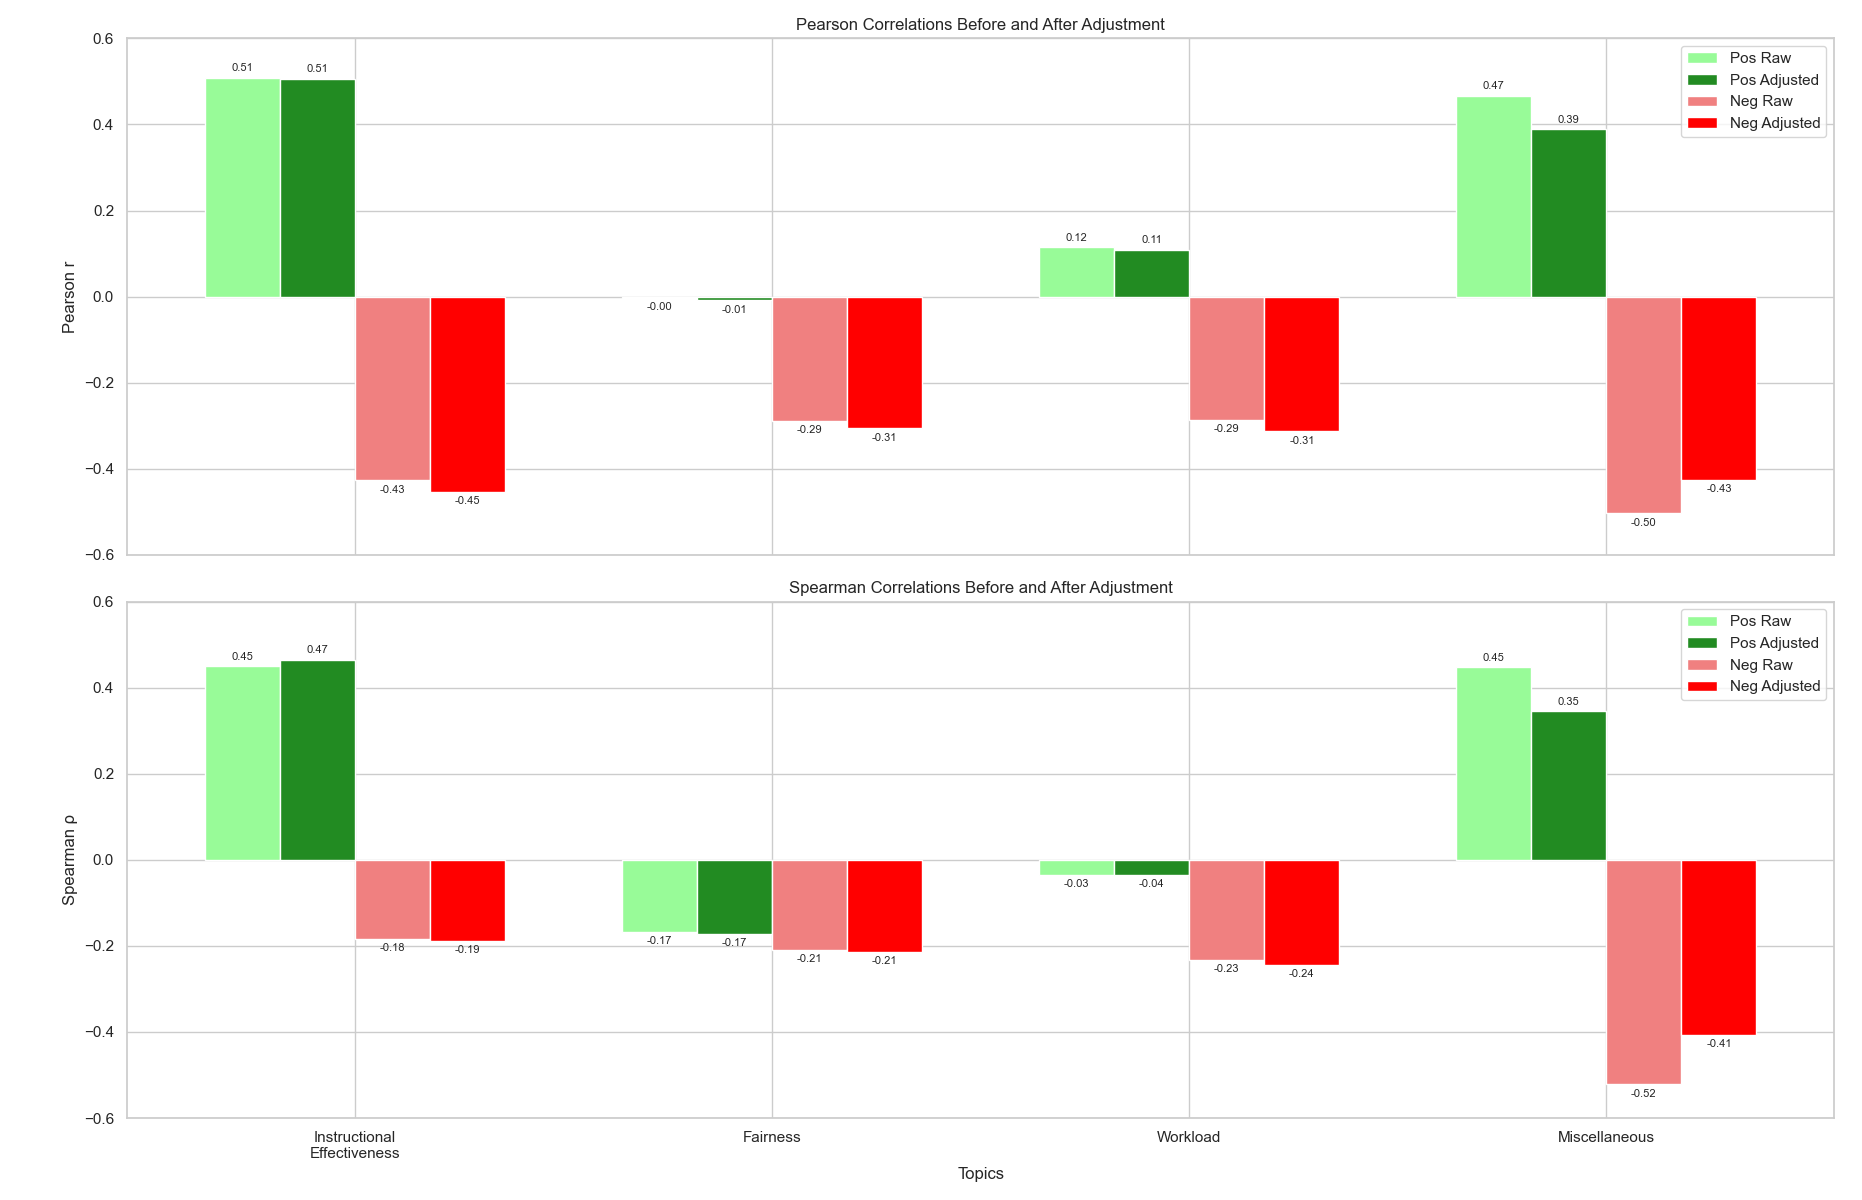
\includegraphics[width=\linewidth]{Diagrams/correlation_changes/pos_neg_corr.png}
    \caption{Pearson and Spearman correlation changes after adjustment, computed on held-out professors ($n = 2{,}052$ reviews).}
    \label{fig:pos-neg-corr-changes}
\end{figure*}

\begin{figure}[H]  
    \centering
    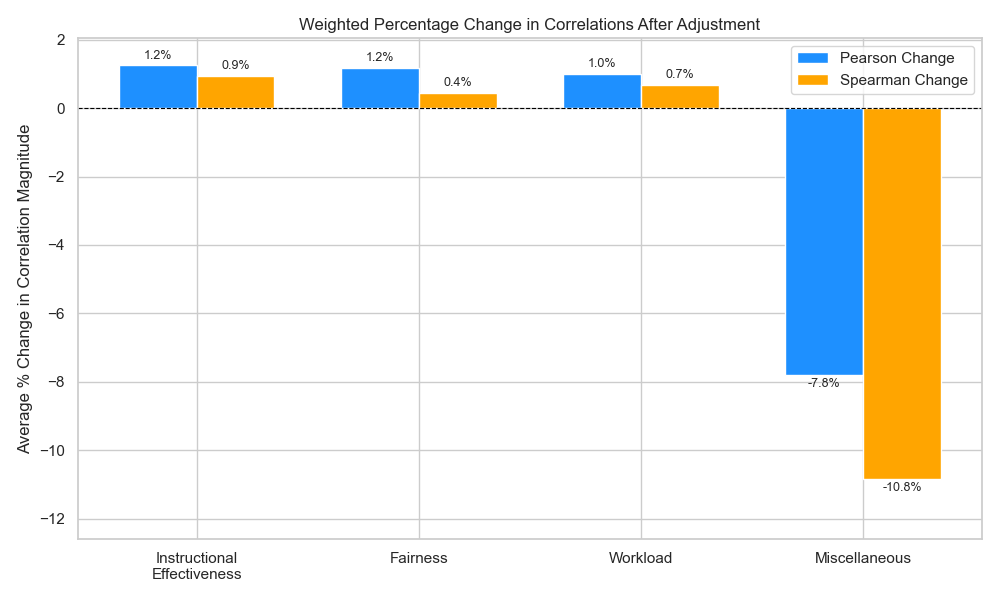
\includegraphics[width=\columnwidth]{Diagrams/correlation_changes/weighted_corr_changes.png}
    \caption{Weighted aggregate Pearson and Spearman correlation changes after adjustment, computed on held-out professors ($n = 2{,}052$ reviews).}
    \label{fig:weighed-corr-change}
\end{figure}

As shown in Figure~\ref{fig:pos-neg-corr-changes} and~\ref{fig:weighed-corr-change} attenuation appears to reduce the correlation of \textit{Miscellaneous} (noise) features with predicted ratings while maintaining or slightly increasing the correlation of pedagogically relevant (signal) features $E_{eff}$, $E_{fair}$ and $E_{work}$. These patterns are consistent across both linear and rank-based correlation measures. Averaged across topics and polarities, signal features tend to show modest increases in correlation magnitude, while noise features tend to decrease, suggesting that adjusted ratings offer a net improvement in the focus on relevant features. These trends align with the intended effect of attenuation and rating adjustment though the precise magnitude of changes may vary across individual features and reviews.
\subsubsection{Modulator Correlations}
\begin{figure*}[btp]  
    \centering
    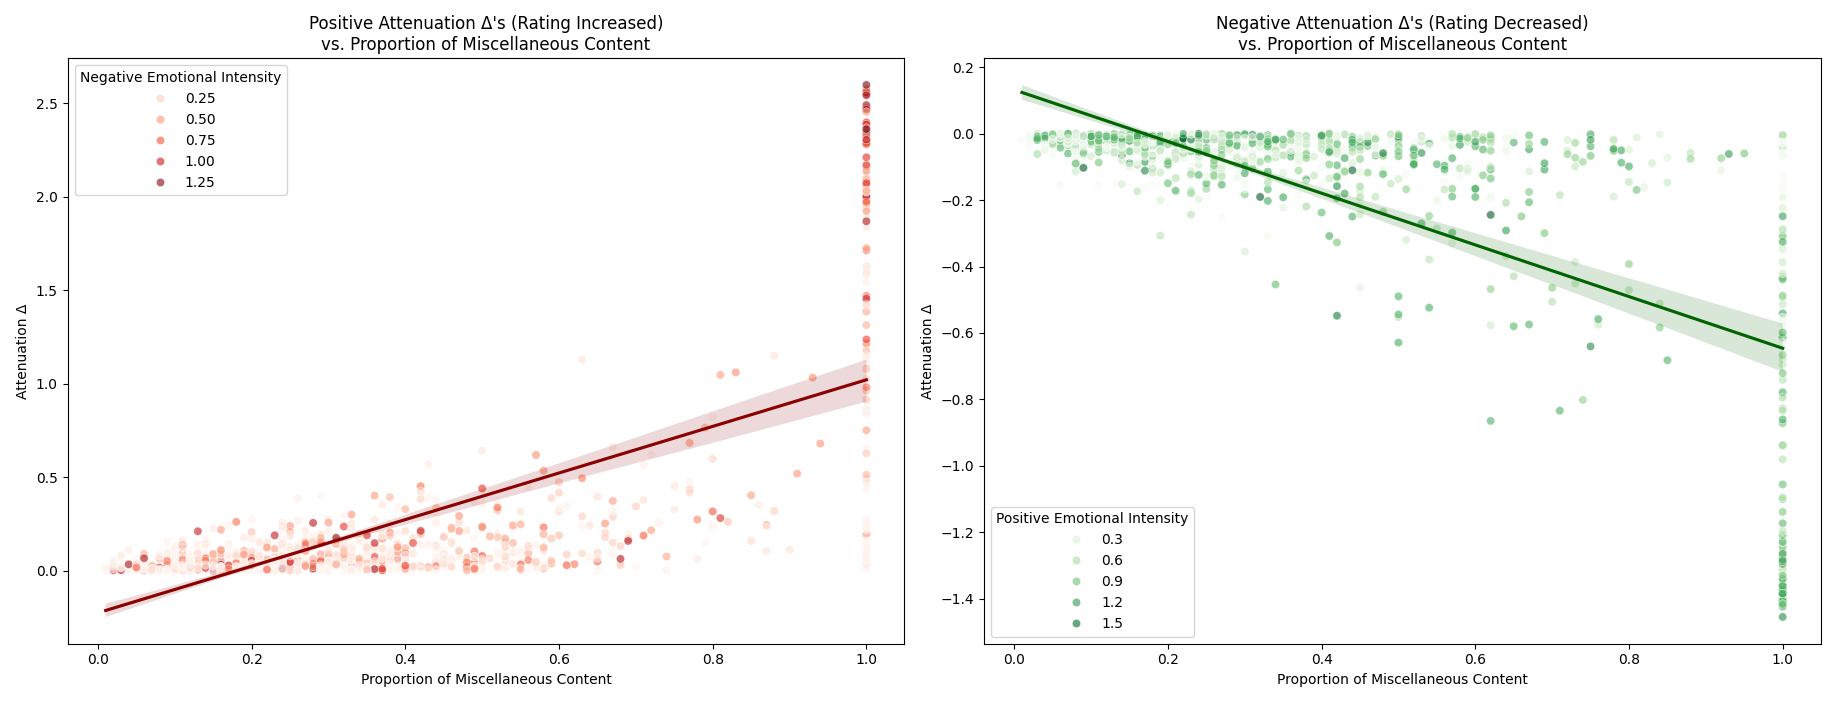
\includegraphics[width=\linewidth]{Diagrams/attenuation_correlation/att-vs-misc.png}
    \caption{Attenuation $\Delta$ versus $D_{misc}$, computed on held-out professors ($n = 2{,}052$ reviews).}
    \label{fig:attvsmisc}
\end{figure*}
To examine how the attenuation mechanism adjusts ratings in response to \textit{Miscellaneous} content, we analyze the relationships between attenuation $\Delta$s and attenuation modulators $D_{misc}$ and the intensity of \textit{Miscellaneous} emotions $E_{misc}$. Positive and negative $\Delta$s are considered separately to capture upward and downward adjustments. These correlations quantify the extent to which each modulator drives the magnitude and direction of rating changes. Figure~\ref{fig:attvsmisc} shows scatter plots of $\Delta$s against $D_{misc}$ with opposing-polarity $E_{misc}$ intensity encoded by color, visually illustrating the systematic relationship between modulator $D_\text{misc}$ and adjustments.

\begin{center}
    \captionof{table}{Correlation analysis: attenuation $\Delta$ versus modulators, computed on held-out professors ($n = 2{,}052$ reviews).}
    \label{tab:correlation_deltas}
    \begin{tabular}{lcc}
    \toprule
    Comparison Relationship & Pearson $r$ & Spearman $\rho$ \\
    \midrule
    $\Delta^+$ vs. $D_{misc}$ & 0.6956 & 0.6218 \\
    $\Delta^-$ vs. $D_{misc}$ & -0.6966 & -0.5607 \\
    \midrule
    $\Delta^+$ vs. Neg. $E_{misc}$  & 0.3600 & 0.4185 \\
    $\Delta^-$ vs. Pos. $E_{misc}$  & -0.2258 & -0.1063 \\
    \bottomrule   
    \end{tabular}
\end{center}

Table~\ref{tab:correlation_deltas} substantiates $D_{misc}$ as the primary and reliable driver of attenuation: ratings tend to increase or decrease in proportion to the modulator, while correlations with $E_{misc}$ intensities are weaker, yet not insignificant. This aligns with expectations. $D_{misc}$ directly controls the weighting strength $\zeta$, meaning that intense \textit{Miscellaneous} sentiment alone does not necessarily produce substantial attenuation.

To further substantiate the proportional nature of attenuation, a Mann-Whitney U test (Wilcoxon rank-sum test) compares absolute adjustment magnitudes between low noise reviews ($D_{misc} < 0.2$, $n=690$) and high noise reviews ($D_{misc} > 0.5$, $n=508$). Results confirm that high noise reviews receive significantly larger absolute adjustments than low noise reviews ($U = 313{,}093$, $p < 0.001$, rank biserial $|r| = 0.786$), with a large effect size. This provides direct empirical evidence that attenuation magnitudes scale proportionally with $D_{misc}$.

\subsubsection{Internal Validation Conclusion}
Internal validation indicates that the attenuation mechanism functions as designed. Feature importance shifts, correlation changes, and attenuation–modulator relationships consistently show that the system reduces the influence of off-topic \textit{Miscellaneous} sentiment while preserving or enhancing sensitivity to core pedagogical signals. These patterns provide evidence that attenuation introduces structured and interpretable adjustments to predicted ratings rather than arbitrary changes.
\subsection{Attenuation Validation - External}
To assess whether the validity-weighted attenuation mechanism produces adjustments that align with human judgment, a senior faculty expert conducted a paired comparison evaluation.

Pairs were constructed in two phases. In the first phase, coarse pairs were formed by randomly sampling one review from a minimal adjustment bin ($|\Delta| < 0.15$) and one from a significant adjustment bin ($|\Delta| \geq 0.65$). In the second phase, fine-grained pairs were constructed by sampling two reviews whose absolute attenuation $\Delta$ differed less than 0.40, producing pairs where the difference in CIV contamination is more subtle. In both phases, reviews were verified for correct ATC categorization prior to inclusion. Presentation order within each pair was randomized.

The expert was presented with the raw textual content of both reviews in each pair, with no access to model outputs, attenuation $\Delta$s, or ATC categorizations. For each pair, the expert was asked to judge which of the two reviews  was more valid for SET. A prediction was considered correct if the review identified as more valid by the expert corresponded to the review receiving the smaller absolute attenuation $|\Delta|$. This tests the assumption that a more pedagogically valid review requires less adjustment. The expert was also able to leave the label section empty, indicating there was no perceivable difference in review validity. Model predictions for these unsure responses were counted as incorrect.

Expert validation is reported over the full sample of adjusted reviews. Pair construction was constrained on two fronts: both reviews had to fall in the required $|\Delta|$ bins, and both had to be verified as correctly categorised by ATC, which limits the pool of eligible pairs. Reporting on the full sample carries no circularity risk in any case, as the expert judged raw review text alone and expert agreement enters none of the criteria used to select $s$.
\begin{center}
    \captionof{table}{Paired comparison accuracy.}
    \label{tab:external-validation}
    \begin{tabular}{lcccc}
    \hline
    \textbf{Condition} & \textbf{\#} & \textbf{Unsure} & \textbf{Corr.} & \textbf{Acc.} \\
    \hline
    ($|\Delta_{1}-\Delta_{2}| \geq 0.5$) & 45 & 3 & 40 & 0.889 \\
    ($|\Delta_{1}-\Delta_{2}| \leq 0.4$) & 29 & 1 & 22 & 0.759 \\
    \hline
    \end{tabular}
\end{center}

Table~\ref{tab:external-validation} shows that the attenuation mechanism is in strong agreement with expert judgment. Under coarse conditions, the framework correctly identified the more valid review 88.9\% of the time, significantly above chance ($p < 0.001$). Performance declined under fine-grained conditions but remained statistically significant (75.9\%, $p < 0.005$). This pattern is consistent with expectations: larger differences in construct-irrelevant content are easier to detect and adjust for than subtle ones. These results suggest that attenuation $\Delta$s effectively signals the presence of emotional CIV, confirming that the framework successfully identifies reviews where strong off-topic sentiment compromises validity. Despite showing promise, these results should be considered preliminary due to reliance on a single expert; future work will expand validation to include multiple independent evaluators.
\section{Results}
Findings across ATC, clause level RoBERTa-GoEmotions sentiment extraction, regression model training, and rating adjustments, are presented next.
\subsection{ATC Topic Structure}
We examine the frequency of topics after ATC. Figure~\ref{fig:topic_freq} shows that at the clause level, \textit{Instructional Effectiveness} is the most mentioned topic in our dataset (25,845), followed by \textit{Miscellaneous} (17,607) and \textit{Workload} (15,683), with \textit{Fairness} trailing substantially behind (4,258). The prominence of \textit{Miscellaneous} clauses indicates that a substantial portion of student discourse falls outside pedagogical dimensions.

\begin{figure}[H]  
    \centering
    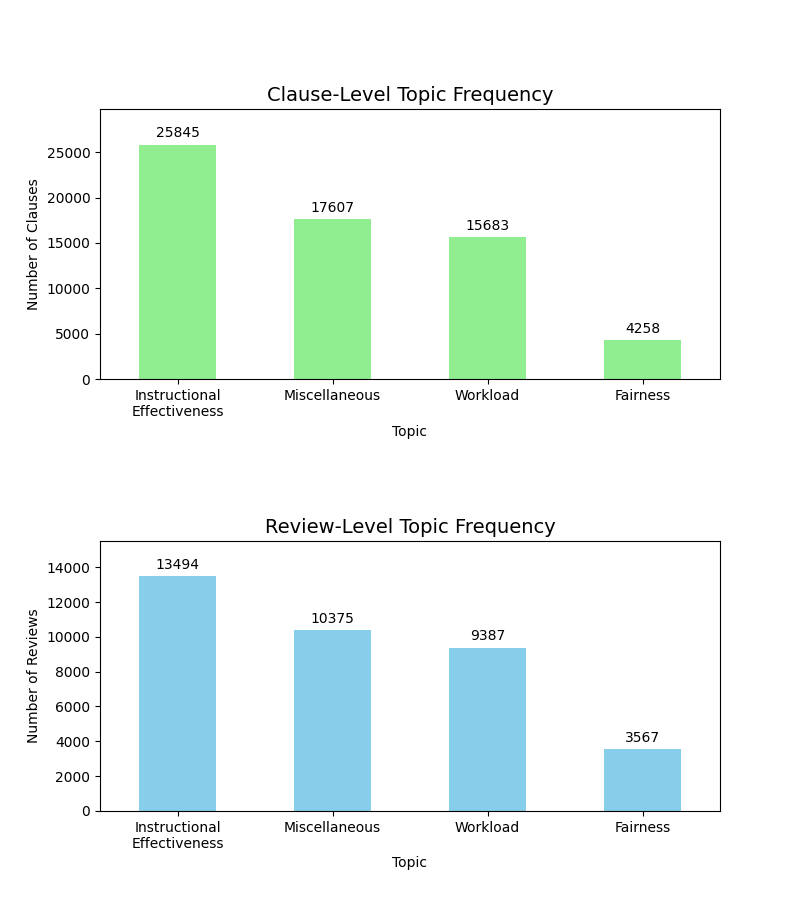
\includegraphics[width=\columnwidth]{Diagrams/atc_visuals/topic-freq.png}
    \caption{Review-level and clause-level topic frequency.}
    \label{fig:topic_freq}
\end{figure}



\begin{table}[H]
\centering
\captionof{table}{Clause and review-level topic frequencies.}
\label{tab:clause_review_freq}
\begin{tabular}{l c}
\toprule
\textbf{Metric} & \textbf{Value} \\
\midrule
\multicolumn{2}{l}{\textit{Instructional Effectiveness}} \\
Clause Frequency & 25,845 \\
Review Frequency & 13,494 \\
Avg. Clauses per Review & \textbf{1.92} \\
\midrule
\multicolumn{2}{l}{\textit{Miscellaneous}} \\
Clause Frequency & 17,607 \\
Review Frequency & 10,375 \\
Avg. Clauses per Review & \textbf{1.70} \\
\midrule
\multicolumn{2}{l}{\textit{Workload}} \\
Clause Frequency & 15,683 \\
Review Frequency & 9,387 \\
Avg. Clauses per Review & \textbf{1.67} \\
\midrule
\multicolumn{2}{l}{\textit{Fairness}} \\
Clause Frequency & 4,258 \\
Review Frequency & 3,567 \\
Avg. Clauses per Review & \textbf{1.19} \\
\bottomrule
\end{tabular}
\end{table}

At the review level, where frequency reflects whether a review contains at least one clause categorized under a given topic, the same overall ordering holds. However, comparison of clause and review-level frequencies reveals differences in clause density across topics (Table~\ref{tab:clause_review_freq}). \textit{Instructional Effectiveness} exhibits the highest average number of clauses per topic-mentioning review (1.92), suggesting that when students discuss instructional quality, they tend to elaborate across multiple clauses. In contrast, \textit{Fairness} displays a substantially lower clause-per-review ratio (1.19), indicating that fairness and grading-related comments are typically more concise or singular in structure. \textit{Miscellaneous} and \textit{Workload} fall between these extremes (1.70 and 1.67, respectively), reflecting moderate elaboration depth.

Examining the frequency of topic combinations (Figure~\ref{fig:topic-combinations}) reveals clear thematic patterns. Reviews that mention only \textit{Instructional Effectiveness} are substantially more common than reviews containing only one of the other three topics. \textit{Workload} rarely appears in isolation and is most often mentioned alongside \textit{Instructional Effectiveness}. A similar pattern is observed for \textit{Miscellaneous} and \textit{Fairness}, which tend to co-occur with \textit{Instructional Effectiveness} rather than appearing alone. These results indicate that \textit{Instructional Effectiveness} functions as a central topic, while other topics are typically discussed in combination with it.

\begin{figure*}[btp]  
    \centering
    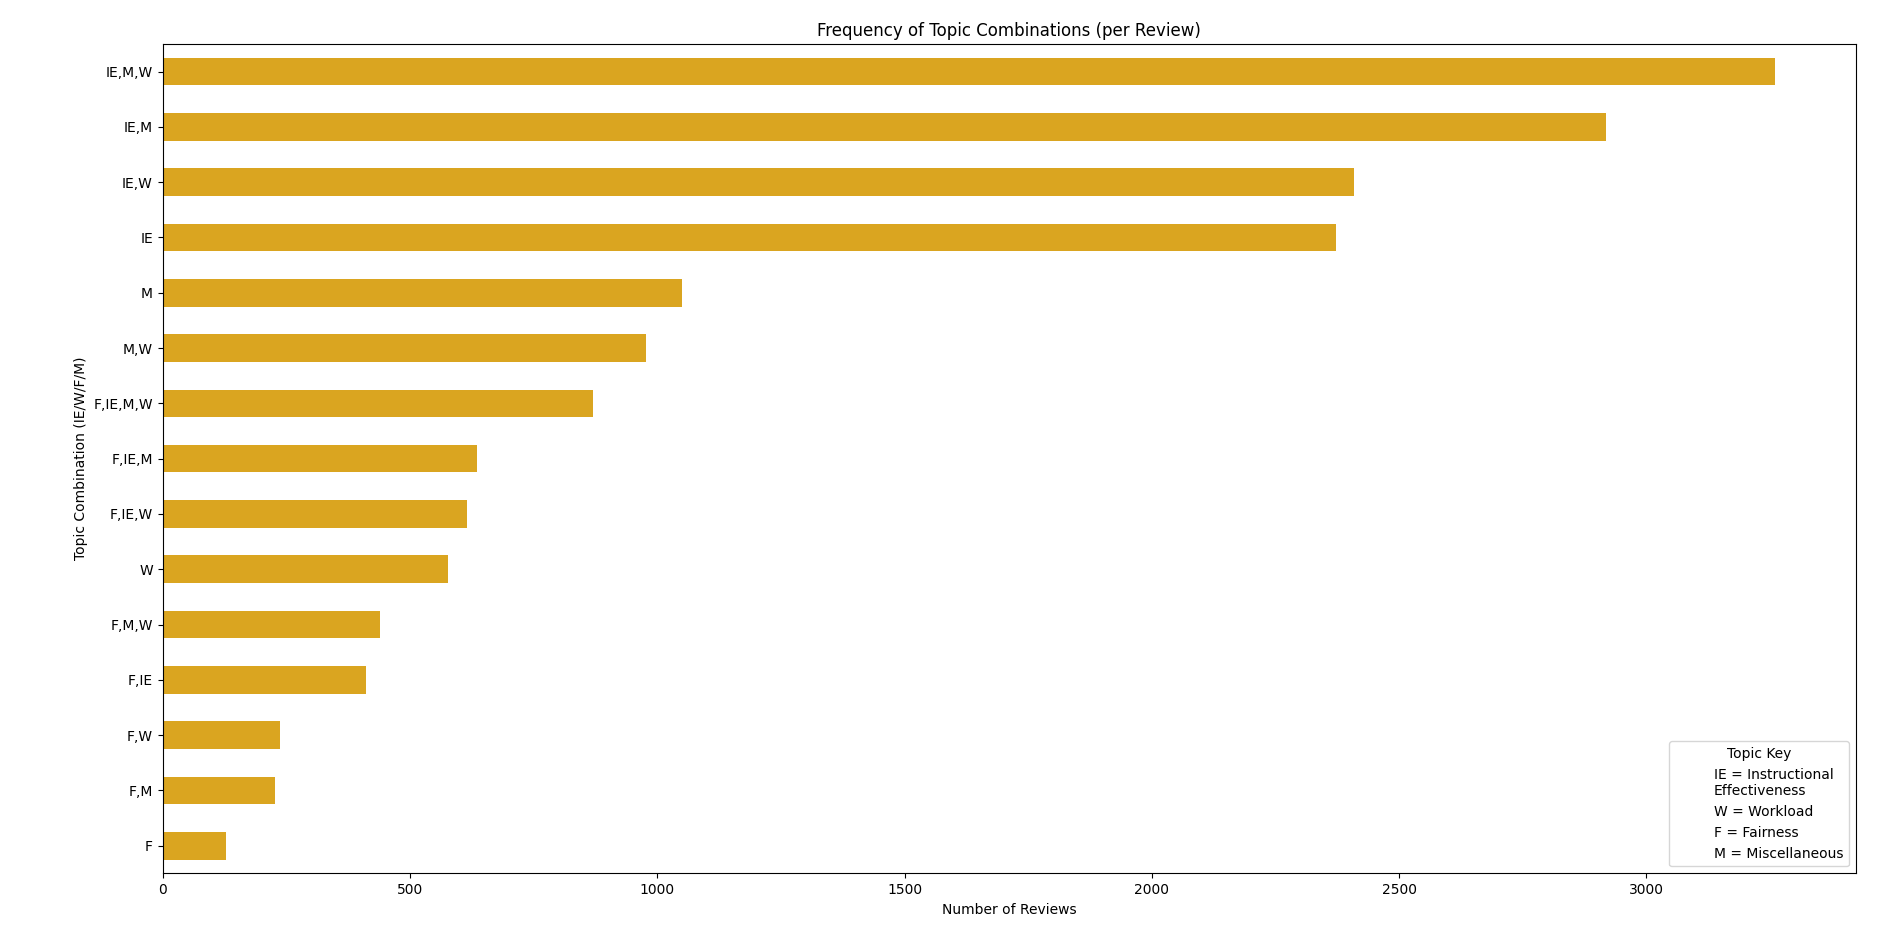
\includegraphics[width=\linewidth]{Diagrams/atc_visuals/topic-combinations.png}
    \caption{Frequency of topic combinations per review.}
    \label{fig:topic-combinations}
\end{figure*}

Figure~\ref{fig:rating-heatmap} presents the frequency of clauses associated with each rating and topic as a heatmap. Clauses from 5-star reviews constitute the majority of all clauses, reflecting the previously observed negative skew in review ratings. Despite this skew, low-rating reviews show notable patterns. For ratings 1.0, 1.5, and 2.0, \textit{Miscellaneous} clauses have the highest absolute counts among the four topics. This is most pronounced for 1-star reviews, where \textit{Miscellaneous} clauses occur approximately 27\% more frequently than the next most frequent pedagogical topic. Additionally, 1-star \textit{Fairness} clauses also appear in relatively high absolute counts, despite the overall predominance of 5-star reviews. 

\begin{figure*}[btp]  
    \centering
    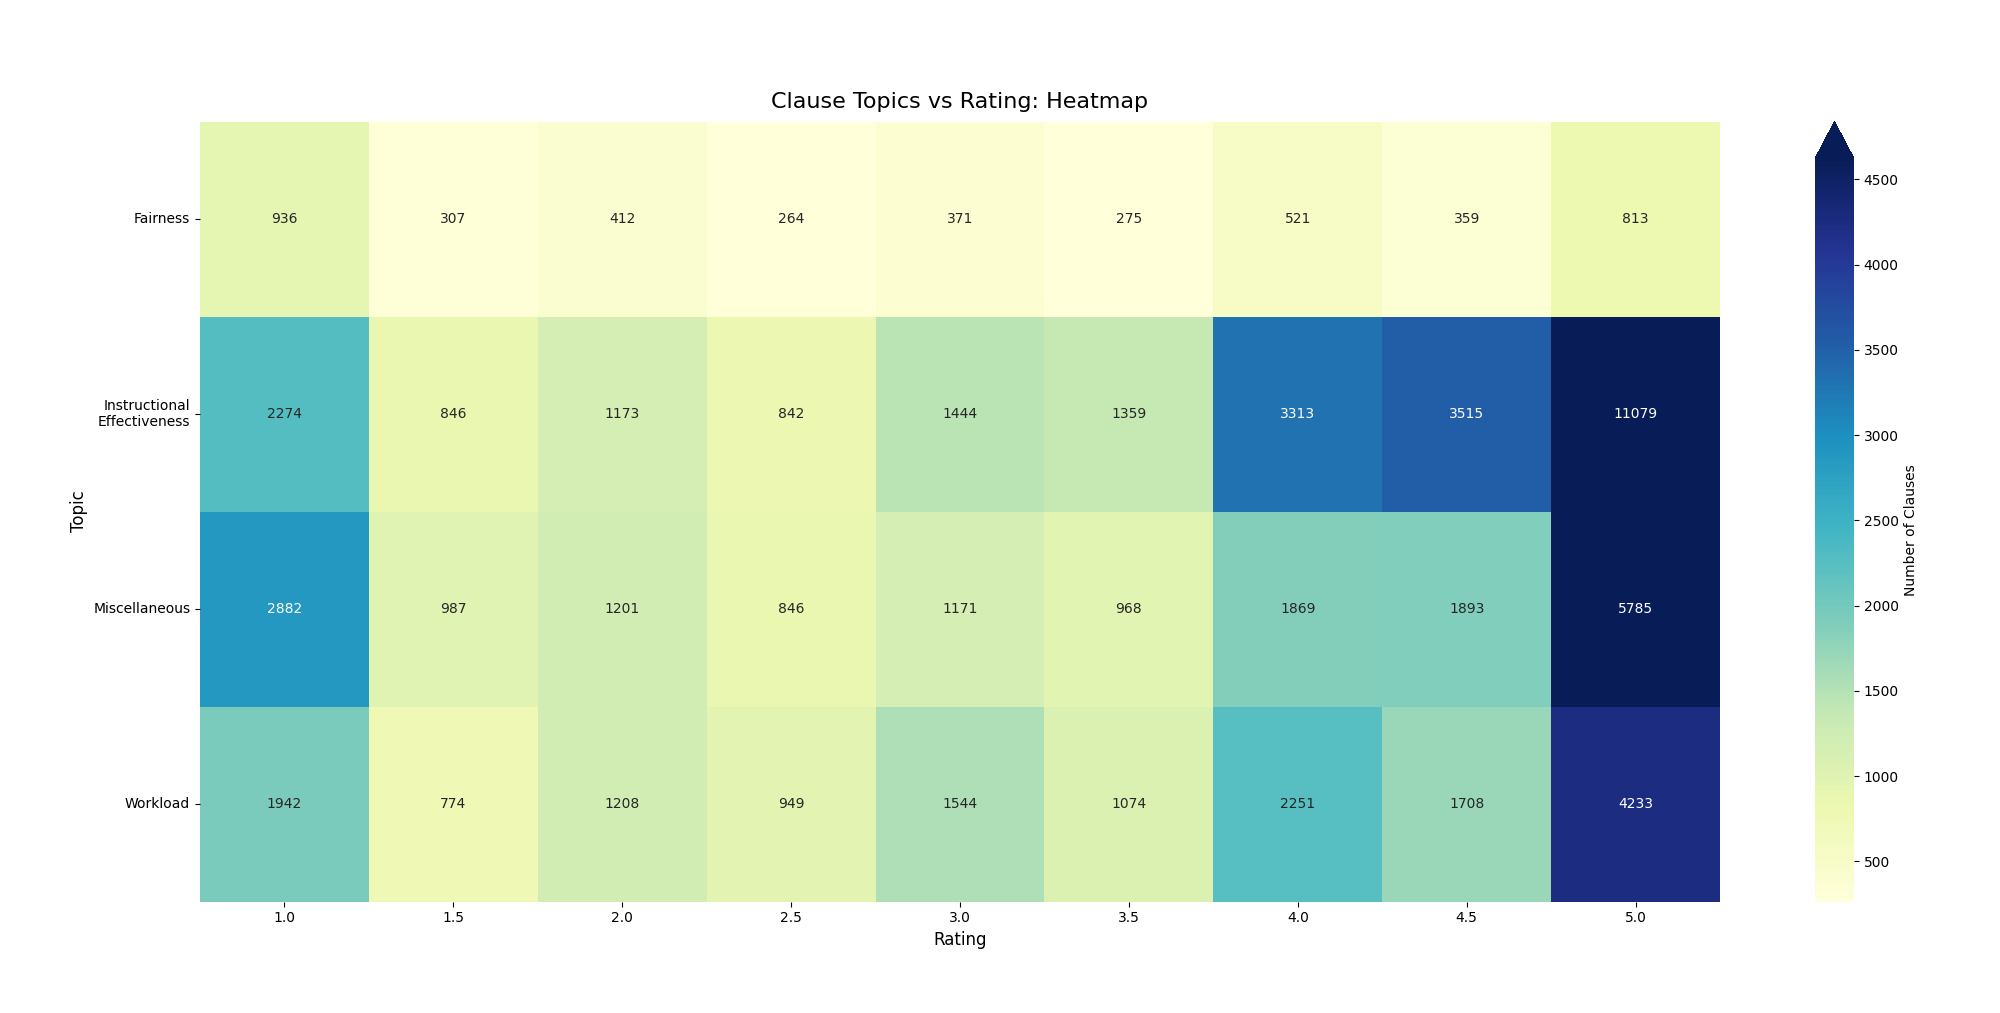
\includegraphics[width=\linewidth]{Diagrams/atc_visuals/topic-rating-heatmap.png}
    \caption{Topic heatmap across ratings.}
    \label{fig:rating-heatmap}
\end{figure*}

\begin{figure*}[btp]  
    \centering
    
\includegraphics[width=\linewidth]{Diagrams/atc_visuals/dmiscdistribution.png}
    \caption{$D_\text{misc}$ distribution across all reviews.}
    \label{fig:dmisc_dist}
\end{figure*}

Finally, Figure~\ref{fig:dmisc_dist} presents the distribution of $D_{\text{misc}}$ across all 
reviews following ATC. The distribution is heavily positively-skewed, with a median of 0.11 
and mean of 0.22, indicating that the majority of reviews contain relatively little 
Miscellaneous content. A notable spike at $D_{\text{misc}}$=1.0 reflects reviews 
composed entirely of non-pedagogical content, a subset that receives maximal attenuation 
under the proposed framework. Miscellaneous content, 
is present across the dataset but varies substantially in density across reviews.

In summary, ATC analysis reveals that \textit{Instructional Effectiveness} dominates both clause and review-level frequencies, and is a central topic in co-occurrence patterns. \textit{Miscellaneous} and \textit{Workload} are moderately frequent, while \textit{Fairness} is comparatively rare, but shows notable representation in low-rating reviews. The distribution of $D_\text{misc}$ across reviews is heavily right-skewed, with the majority of reviews containing relatively low proportions of Miscellaneous content, though a non-trivial tail of high-density and fully Miscellaneous reviews motivates the proportional rather than uniform attenuation design. Together, these results provide a structural overview of topic distributions, thematic patterns across ratings, and the distribution of pedagogical noise that the subsequent attenuation procedure is designed to mitigate.

\subsection{Sentiment Extraction (RoBERTa)}
RoBERTa-GoEmotions sentiment extraction reveals distinct emotional signatures within clauses. To manage the high dimensionality of the output vectors, the findings are presented as heat maps, showing only the ten emotions with the highest mean probability.

For all clauses (Figure~\ref{fig:emotional-heatmap}) positive emotions are on average more common than negative emotions. This is likely a symptom of the dataset due to the negative skew in the rating distribution. Notably, positive sentiments towards \textit{Instructional Effectiveness} are the dominant emotional signal in student reviews clauses. Furthermore, total emotional signal directed towards pedagogical categories is on average stronger than that directed towards \textit{Miscellaneous}. However, this claim weakens when comparing \textit{Miscellaneous} individually to other topics.

Examining the clauses associated with 5-star reviews (Figure~\ref{fig:5star-emotional-heatmap}), we observe that positive emotions directed towards all four topics constitute the bulk of the emotional signal for 5-star reviews. \textit{Miscellaneous} sentiment tends to have strong probability for positive emotions approximately equal to that of \textit{Fairness} and \textit{Workload}, yet weaker than \textit{Instructional Effectiveness} in general. Interestingly, love and amusement are the only emotions for which \textit{Miscellaneous} is the highest-probability topic.

Moving on to 1-star clauses (Figure~\ref{fig:1star-emotional-heatmap}), pedagogical topics generally exhibit equal or greater emotional density relative to \textit{Miscellaneous}. The overall range and maximum of probabilities are lower than in 5-star clauses, reflecting more concentrated and less intense emotional expression. Within 1-star clauses, \textit{Miscellaneous} exhibits relatively stronger signals compared to other topics, even though its absolute probabilities remain equal to or lower than than those of pedagogical topics.

Comparing 1-star and 5-star clauses reveals two notable trends. First, both extremes of the rating spectrum contain emotional outliers of the opposite valence: 1-star clauses occasionally exhibit positive emotions, while 5-star clauses occasionally include negative emotions. This observation demonstrates that student reviews are not purely unidimensional in their affective content. Second, the emotional probabilities in 1-star clauses are more evenly distributed across numerous emotions, compared to 5-star clauses where the vast majority of the emotional signal is concentrated in admiration and approval.

In summary, the RoBERTa-GoEmotions analysis reveals that student reviews exhibit structured emotional patterns. While \textit{Miscellaneous} emotional probability is consistently weaker than \textit{Instructional Effectiveness}, it occasionally exceeds \textit{Fairness} or \textit{Workload} individually. Positive emotions dominate in high-rated clauses, while negative emotions are concentrated in low-rated clauses. However, both extremes of the rating spectrum contain cross-valence emotional signals. Comparatively 1-star clauses display a more evenly distributed emotional profile compared to the concentrated signals in 5-star clauses. Overall, these patterns suggest that student affect is nuanced and multi-dimensional, with implications for sentiment-based rating analysis and attenuation frameworks.
\begin{figure*}[btp]
    \centering
    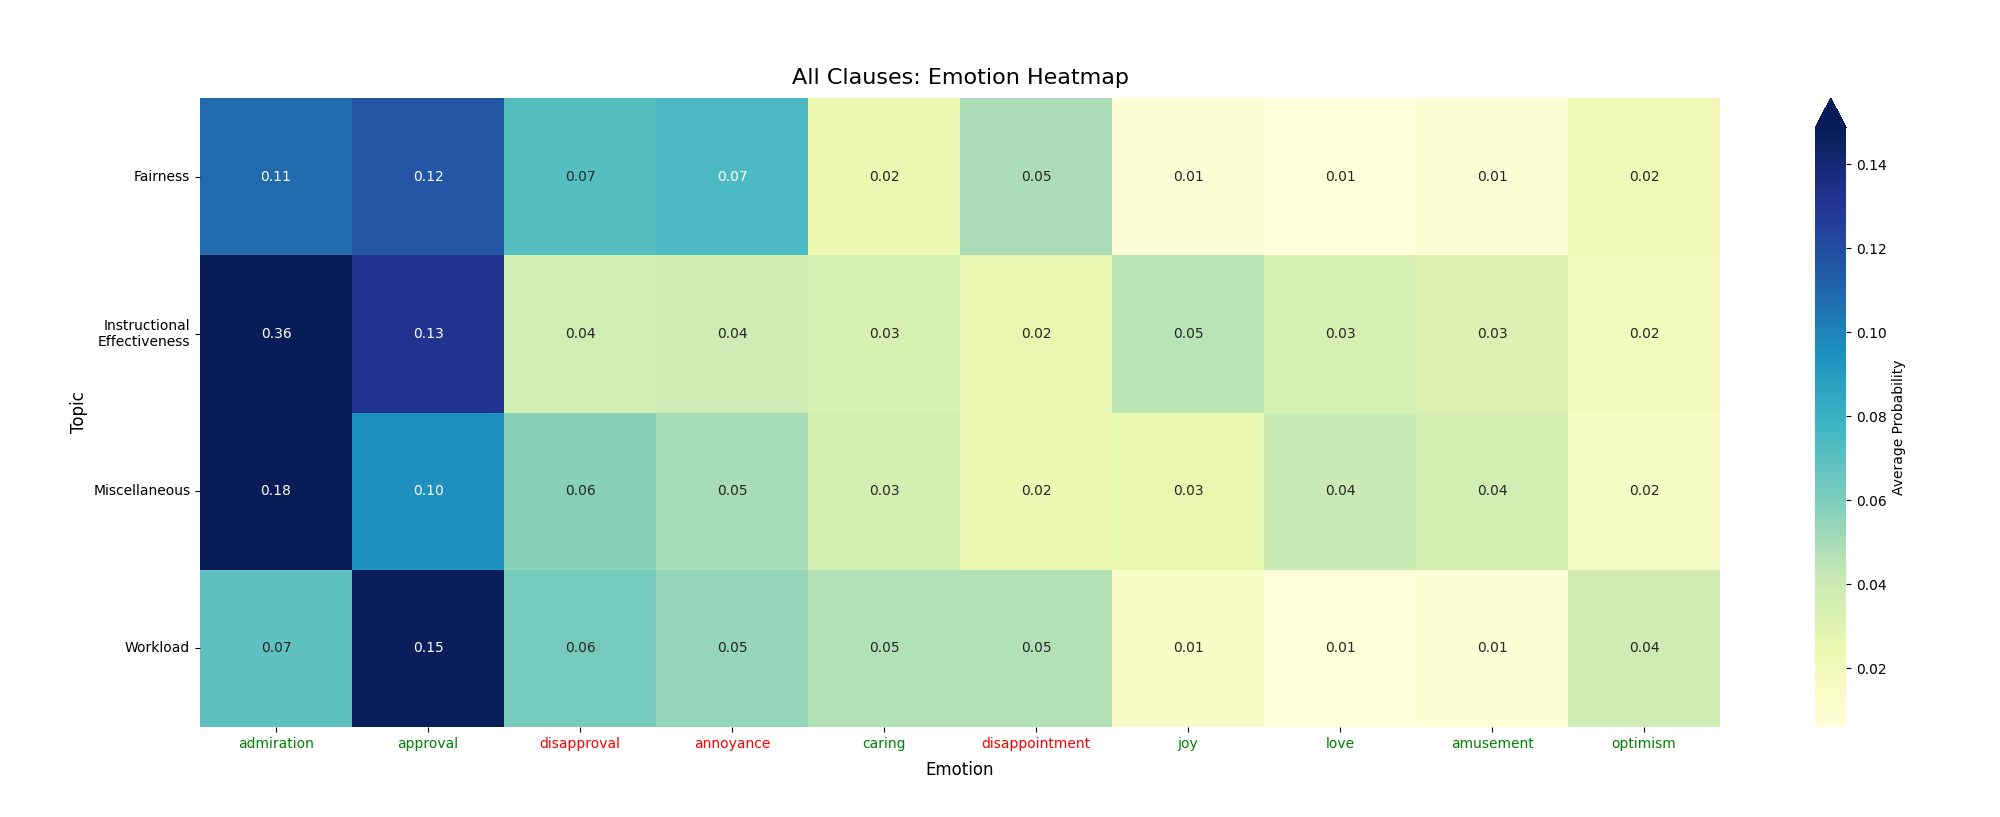
\includegraphics[width=\linewidth]{Diagrams/roberta/all_heatmap_emotions.png}
    \caption{Emotional heatmap of topics.}
    \label{fig:emotional-heatmap}
\end{figure*}
\begin{figure*}[btp]
    \centering
    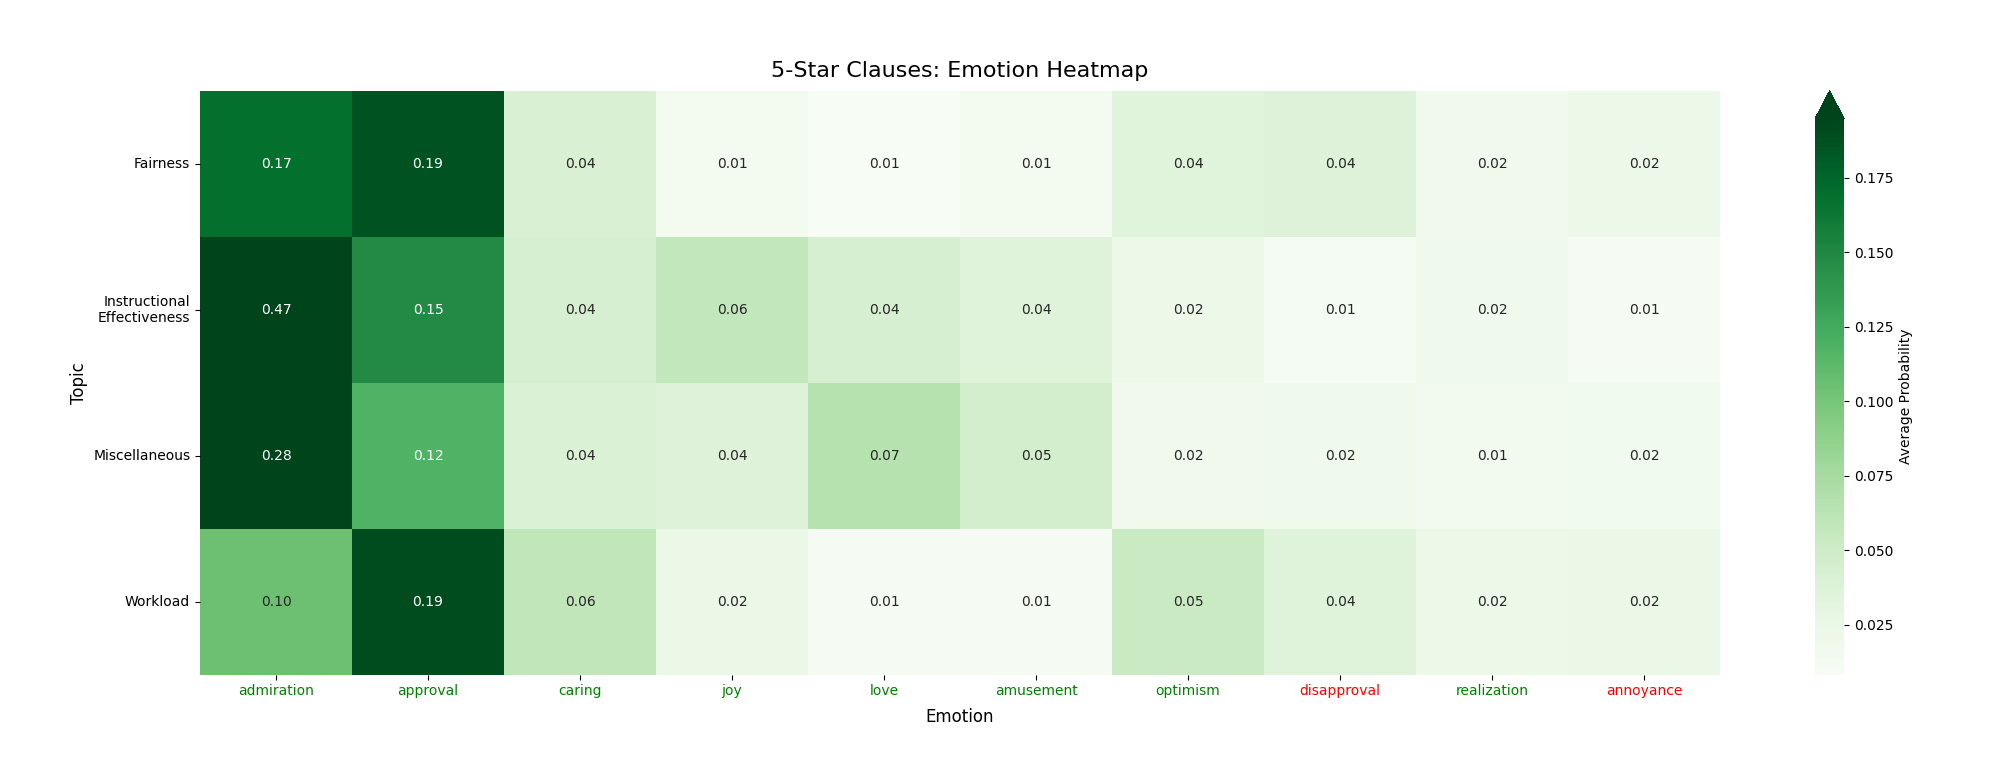
\includegraphics[width=\linewidth]{Diagrams/roberta/5_star_heatmap_emotions.png}
    \caption{Emotional heatmap of topics for 5-star clauses.}
    \label{fig:5star-emotional-heatmap}
\end{figure*}
\begin{figure*}[btp]
    \centering
    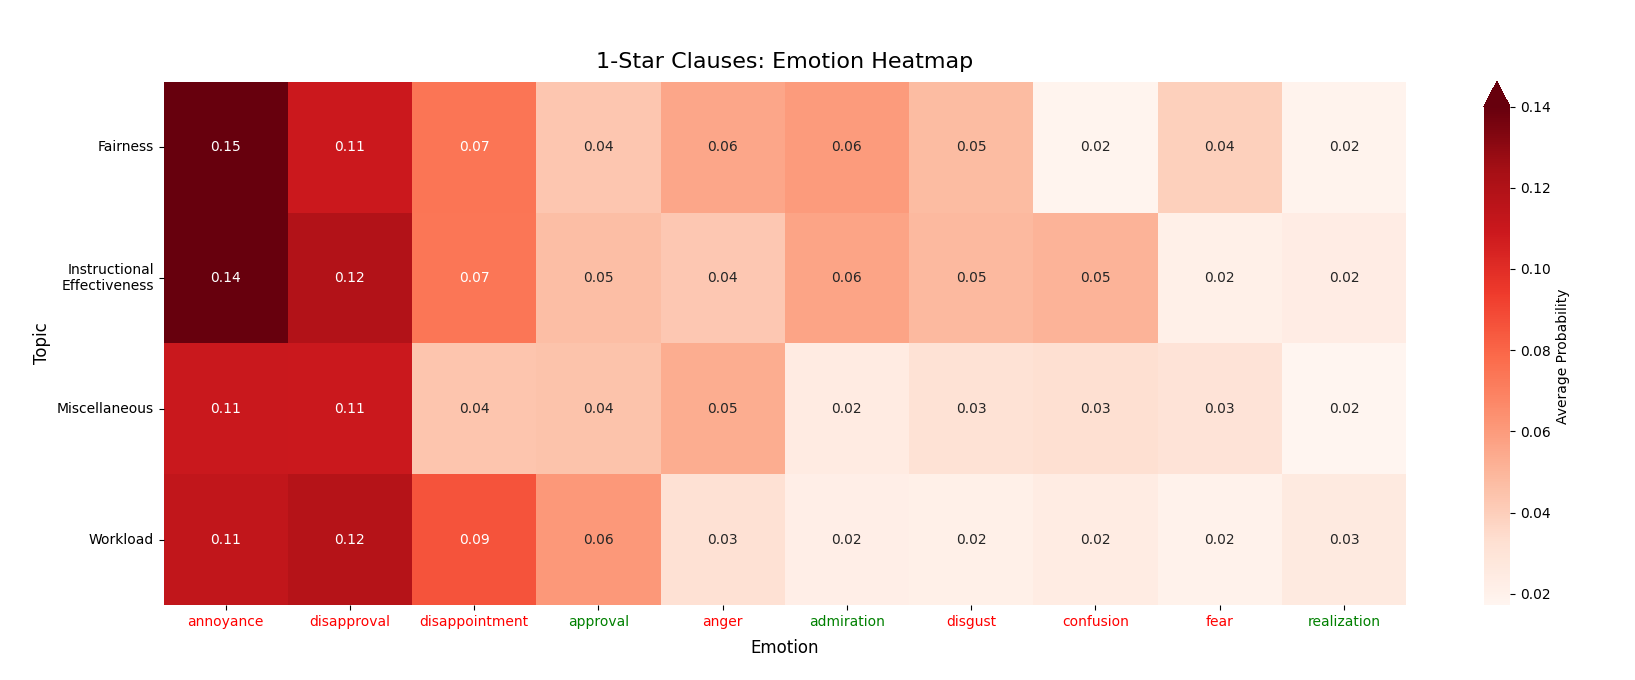
\includegraphics[width=\linewidth]{Diagrams/roberta/1_star_heatmap_emotions.png}
    \caption{Emotional heatmap of topics for 1-star clauses.}
    \label{fig:1star-emotional-heatmap}
\end{figure*}
\subsection{Rating Regression Performance}
Using a professor-level grouped train–test split, the selected CatBoost regressor achieves stable performance across evaluation metrics, indicating reasonable accuracy in predicting numerical ratings from topic-specific emotional features. Table~\ref{tab:CatBoost-performance} lists the final CatBoost model metrics.\newline

\begin{center}
    \captionof{table}{CatBoost regression performance.}
    \label{tab:CatBoost-performance}
    \begin{tabular}{lllc}
    \hline
    \textbf{MAE} & \textbf{$\rho$} & $\textbf{$R^2$}$ \\
    \hline
    0.6369  & 0.7355 & 0.6140\\
    \hline
    \end{tabular}
\end{center}

The final model demonstrates low absolute error, strong ordinal consistency, and substantial explained variance on held-out data, suggesting that it captures meaningful relationships between emotional content and student ratings. 

\subsection{Adjustment Outcomes}
We report summary statistics and distributions at both the review and professor level to provide a quantitative and descriptive overview of how student and professor-level ratings were impacted by the attenuation framework.

Table~\ref{tab:adjustment-stats} presents summary statistics of the rating adjustments performed using the sentiment-aware attenuation framework. Overall, 10,380 ratings were adjusted, corresponding to 60.59\% of all ratings in the dataset. The average change ($\Delta$) across adjusted ratings was 0.0404, with an average absolute change ($|\Delta|$) of 0.2072. Extreme adjustments indicate a maximum positive change of 2.6068 and a maximum negative change of -1.4581, while the smallest nonzero absolute change observed was $2.84\times10^{-6}$. These statistics provide an overview of the magnitude and frequency of adjustments applied at the review level.

\begin{center}
\captionof{table}{Adjustment summary statistics.}
\label{tab:adjustment-stats}
\begin{tabular}{l c}
\toprule
\textbf{Metric} & \textbf{Value} \\
\midrule
\multicolumn{2}{l}{\textbf{Overall Adjustment}} \\
Total Ratings Adjusted & 10380 \\
Percentage of Ratings Adjusted & 60.59\% \\
\midrule
\multicolumn{2}{l}{\textbf{Average Changes}} \\
Average $\Delta$ & 0.0404 \\
Average $|\Delta|$ & 0.2072 \\
\midrule
\multicolumn{2}{l}{\textbf{Extreme Values}} \\
Maximum $\Delta$ & 2.6068 \\
Minimum $\Delta$ & -1.4581 \\
Minimum $|\Delta|$ & $2.84\times10^{-6}$ \\
\bottomrule
\end{tabular}
\end{center}

A Wilcoxon signed-rank test was performed to evaluate whether the observed shifts are systematically different from zero across adjusted reviews. Results indicate a statistically significant shift ($W = 24{,}677{,}804$, $p < 0.001$).

The distribution of individual rating adjustments ($\Delta$) is shown in Figure~\ref{fig:att-distribution}. The majority of adjustments are small, while a long tail extends toward both negative and positive extremes. Positive adjustments tend to reach slightly higher magnitudes than negative adjustments.

Professor-level average rating changes are illustrated in Figure~\ref{fig:prof-distribution}. Two distributions are shown: one for the original average ratings and one for the adjusted averages. The y-axis measures probability density, representing the relative concentration of professors at each rating level. The adjusted averages are generally less dense than the original at the extremes, but more dense across intermediate ranges. The mean professor average increases minimally. Overall, both distributions are negatively skewed, reflecting the predominance of 5-star ratings in the original dataset.

The 20 largest positive and negative changes in professor average ratings are presented in Figure~\ref{fig:largest-prof}. These adjustments are relatively similar in magnitude (approximately $\pm$0.4-0.7), with one moderate outlier among the negative changes.

\begin{figure*}[btp]  
    \centering
    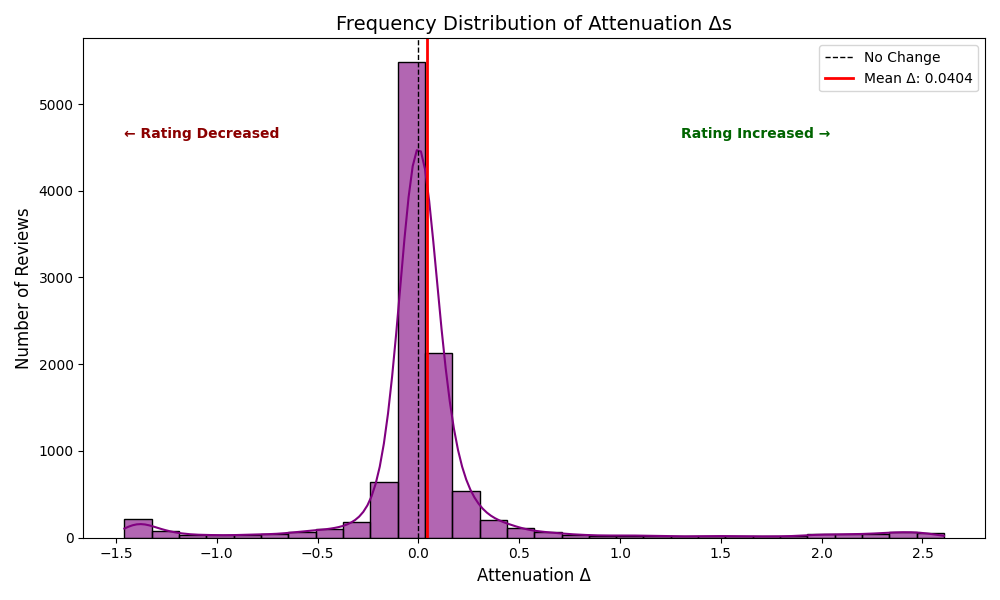
\includegraphics[width=\linewidth]{Diagrams/adjustment_visuals/attenuation-distribution.png}
    \caption{Attenuation $\Delta$ distribution.}
    \label{fig:att-distribution}
\end{figure*}
\begin{figure*}[btp]  
    \centering
    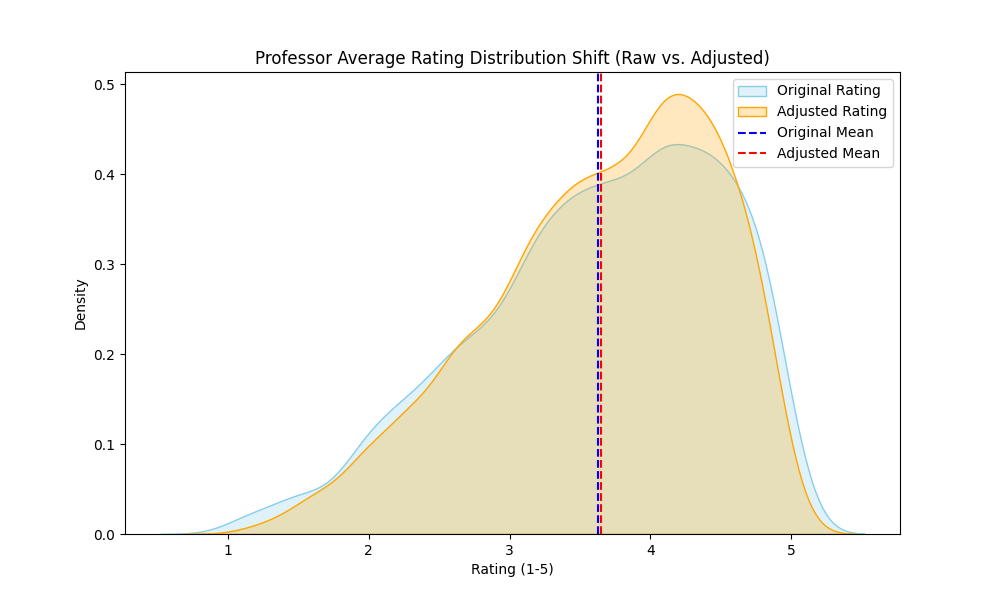
\includegraphics[width=\linewidth]{Diagrams/adjustment_visuals/prof-average-distribution.png}
    \caption{Distribution of professor average rating changes.}
    \label{fig:prof-distribution}
\end{figure*}
\begin{figure}[H]  
    \centering
    
\includegraphics[width=\columnwidth]{Diagrams/adjustment_visuals/largest-prof-changes.png}
    \caption{Largest professor average rating changes (Positive and Negative).}
    \label{fig:largest-prof}
\end{figure}

Overall, these results provide a quantitative overview of the impact of the validity-weighted adjustment procedure. Adjustments at the review level were generally small, with occasional significant targeted adjustments. At the professor level, changes were also moderate to minimal, with somewhat greater impacts observed at the extremes of the rating scale. Despite these adjustments, the overall distribution of professor average ratings remained largely consistent, showing high similarity before and after validity-weighted adjustments.

\section{Discussion}
This research presents a transparent, aspect-based sentiment analysis (ABSA) framework to address construct-irrelevant variance (CIV) in Student Evaluations of Teaching (SET). The findings suggest that while student ratings are strongly influenced by pedagogical factors, they remain susceptible to noise from non-pedagogical emotional content. The proposed validity-weighted attenuation mechanism offers a proof-of-concept for mitigating this type of bias. The framework applies statistical principles and concepts from psychometric validity theory to adjust ratings in an interpretable way.

\subsection{Pedagogical Signal \& Affective Noise}
The results regarding RQ1 reveal a clear relationship between pedagogical feedback and numerical ratings. \textit{Instructional Effectiveness} emerged as the most frequent and influential pedagogical topic, exhibiting the highest review elaboration depth (1.92 clauses per review on average), the strongest emotional intensities when mentioned, and the highest mean SHAP value. While \textit{Workload} was the second most frequent pedagogical topic, its contribution to ratings was more variable, and \textit{Fairness}, though less frequent overall, showed distinct behaviour in low-rating contexts.

The emotional heatmap analysis reveals a distinct asymmetry in how these topics emotionally correspond with ratings at opposing ends of the spectrum. For 5-star reviews, admiration and approval directed towards \textit{Instructional Effectiveness} constituted the dominant emotional signal. In contrast, 1-star reviews exhibited a diffuse emotional profile, where negative emotions such as annoyance, disapproval, and disappointment were spread across all topics, including non-pedagogical ones. Notably, the disproportionately high representation of \textit{Fairness} clauses in low-rating reviews further suggests that perceived fairness and grading inequity may be a higher impact concern among heavily dissatisfied students. This asymmetry suggests that high ratings are driven by concentrated positive affect toward \textit{Instructional Effectiveness}, while low ratings reflect broader, more distributed dissatisfaction.

SHAP analysis of the baseline model shows that Positive \textit{Instructional Effectiveness} was the dominant driver of predicted ratings, followed by Negative \textit{Instructional Effectiveness}, Negative \textit{Miscellaneous}, and Negative \textit{Workload}, with Positive \textit{Fairness} and Positive \textit{Workload} contributing the least. These patterns confirm that emotional responses to pedagogical topics, particularly those directed towards \textit{Instructional Effectiveness}, are the primary systematic drivers of rating variation, answering RQ1.


Analysis also reveals the substantial contribution of non-pedagogical emotional content to numerical ratings, directly addressing RQ2. These results align with Messick’s (1995) concept of CIV: construct-irrelevant content is not only present in informal SET reviews but contributes to numerical ratings in ways often unrelated to instructional quality. While derived from RMP data, this finding is consistent with the broader validity concerns documented in formal SET contexts (Marsh \& Roche, 1997; Langbein, 1994; Schiekirka \& Raupach, 2015). 

The ATC results demonstrated that \textit{Miscellaneous} content constitutes a large share of student reviews, particularly in low-rating contexts where it was the most frequent clause category, occurring approximately 27\% more frequently than the next most common pedagogical topic in 1-star reviews. Furthermore, the distribution of $D_\text{misc}$ across all reviews, while heavily right-skewed with a median of 0.11, reveals a non-trivial proportion of reviews with substantial Miscellaneous content density, confirming that affective noise is a recurring feature of informal SET data. 

The baseline regression model showed that emotions directed towards \textit{Miscellaneous} topics ($E_{misc}$) carry substantial feature importance (mean SHAP $= 0.671$). Specifically, Negative \textit{Miscellaneous} ranked third overall behind only Positive and Negative \textit{Instructional Effectiveness}, and exceeding the contributions of both \textit{Fairness} and \textit{Workload} in either polarity. Positive \textit{Miscellaneous} sentiment ranked fifth, further confirming that non-pedagogical emotional content influences predicted ratings in both directions. This supports observations that SET scores frequently capture student satisfaction or affective noise rather than instructional quality (Dowell \& Neal, 1983; Wongsurawat, 2011). It also aligns with qualitative findings that students' evaluative responses reflect emotional and relational states extending beyond pedagogical experiences (Li et al., 2025).

Together, the findings for RQ1 and RQ2 offer context for interpreting ratings at different points on the rating scale. High ratings exhibit a favourable signal-to-noise ratio because the pedagogical signal, particularly toward \textit{Instructional Effectiveness}, is so strong; however, the absolute amount of \textit{Miscellaneous} emotional noise remains high. Low ratings present a different issue: while absolute emotional contributions are lower across all topics, \textit{Miscellaneous} sentiment makes up a proportionally larger share of the signal. Across both extremes, the SHAP analysis confirms that \textit{Miscellaneous} emotions remain among the top contributors to predicted ratings overall. Consequently, construct-irrelevant noise contaminates ratings across the entire spectrum, motivating the need for interpretable attenuation mechanisms that address these variations without excluding data.

\subsection{Effectiveness of Validity-Weighted Attenuation}

Addressing RQ3, the results of internal and external validation provide tentative evidence that the proposed attenuation mechanism can attenuate the influence of CIV while preserving much of the pedagogical signal contained in the reviews. The strong performance of the regression model ($\rho = 0.7355$, $R^2 = 0.6140$) confirms that numerical ratings are not arbitrary and are predictable functions of emotions expressed towards specific review topics. The internal validation results were particularly telling: following attenuation of $E_{misc}$, SHAP-based feature importance shifted away from \textit{Miscellaneous} sentiment ($-10.8\%$) and toward core pedagogical categories (\textit{Instructional Effectiveness}: $+2.0\%$; \textit{Fairness}: $+2.7\%$; \textit{Workload}: $+2.6\%$). This suggests that when construct-irrelevant signals are down-weighted, the model relies more heavily on pedagogical features when predicting ratings.

Crucially, the correlation analysis revealed that attenuated ratings maintained or strengthened correlations with pedagogical emotions ($E_{eff}$, $E_{fair}$, $E_{work}$) while reducing correlations with non-pedagogical emotions ($E_{misc}$). This statistical separation suggests that the framework works as intended. Unlike simple data-exclusion approaches, this method applies proportional down-weighting based on the density of irrelevant content ($D_{misc}$). The raw student rating is preserved throughout, with the adjustment adding only the model-estimated correction for construct-irrelevant sentiment. Reviews with predominantly pedagogical content receive minimal adjustment, while those with high \textit{Miscellaneous} density and emotionally polarized irrelevant content receive larger adjustments. 

The attenuation correlation analysis supports the internal coherence of the adjustment mechanism, confirming that its behaviour is systematic. Positive and negative rating $\Delta$s correlate substantially with $D_{misc}$ ($r = 0.696$ and $r = -0.697$, respectively). Although this relationship is partly expected given that $D_{misc}$ directly controls the weighting factor $\zeta$, the pattern confirms that adjustment magnitudes generally scale proportionally with measured noise density rather than reflecting arbitrary variation. The moderate divergence between Pearson and Spearman correlations ($\rho = 0.622$, $\rho = -0.561$) suggests that a subset of reviews with extreme \textit{Miscellaneous} density and high emotional polarization produce large adjustments that inflate the linear correlation, while the rank-based relationship is more conservative. This observation is consistent with the long-tailed distribution of attenuation $\Delta$s observed in Figure~\ref{fig:att-distribution}. 

The weaker but non-negligible correlations between attenuation $\Delta$s and \textit{Miscellaneous} emotional intensity ($r = 0.360$ and Spearman $\rho = 0.419$ for $\Delta^+$ vs. negative $E_{misc}$; $r = -0.226$ and $\rho = -0.106$ for $\Delta^-$ vs. positive $E_{misc}$) further indicate that adjustment magnitude is sensitive to both the proportion of irrelevant content and the emotional intensity within it. The correlation asymmetry between upward and downward corrections and $E_\text{misc}$ intensity warrants further investigation.

At the review level, the average absolute rating change was $0.2072$ rating points, with a tail of larger targeted adjustments for reviews exhibiting high \textit{Miscellaneous} density and intense off-topic emotional polarization. At the professor level, the overall distribution shape remained largely preserved. These results suggest that the framework functions as a fine-tuning mechanism, correcting the most severe instances of CIV contamination while aiming to preserve valid student feedback. This behavior aligns with the conservative correction strategy advocated by Marsh and Roche (1997).

In summary, these results suggest that validity-weighted attenuation can mitigate the influence of CIV while preserving pedagogical signal, providing evidence to address RQ3.

\subsection{Theoretical \& Practical Implications}

This work extends prior descriptive SET studies by presenting a proof-of-concept framework for active mitigation of validity threats, motivated primarily by Messick's (1995) unified theory of validity. The framework uses classical reliability theory (Cronbach, 1951; Huber, 1964) to justify the down-weighting approach. The adjustment process is made transparent by holding the trained model fixed while applying a targeted intervention to $E_\text{misc}$, with the resulting prediction difference taken as the validity correction.. This connects traditional psychometric validity concepts with modern computational NLP methods. It addresses the same validity threats targeted by Zhai et al. (2021), who demonstrate CIV reduction in controlled constructed-response assessments, to the considerably more challenging setting of informal, anonymous, and unmoderated SET reviews. In doing so, it prioritizes interpretability and transparency as essential design constraints, in contrast to the growing reliance on black-box systems in the domain (Zhuang et al., 2025; Rybinski \& Kopciuszewska, 2021).

In its current form, the framework has notable practical implications for student-facing platforms. For informal platforms like RMP, the framework provides a mechanism to increase the trustworthiness of ratings. Adjusted ratings could serve as a more reliable signal for students scanning overall scores to select courses or professors. Topic-level insights might allow users to differentiate between differing emotional reactions to professors in areas such as \textit{Fairness} versus \textit{Workload}.

More broadly, these findings demonstrate that informal SET ratings are systematically distorted by non-pedagogical noise, potentially misinforming the real educational decisions of students who rely on platforms like RMP. This demonstrated susceptibility to affective noise highlights the risk of relying on raw scores in any evaluative context. For institutions processing formal SET data, the methodology suggests a direction for future validity-aware frameworks suitable for consequential institutional use, if rigorously advanced and tested. In addition, SHAP-based and topic-level emotional analysis might offer important insights for faculty development. For example, the dominance of \textit{Instructional Effectiveness} as a predictor could indicate institutional prioritization of improvements in instructional delivery, while the disproportionate representation of \textit{Fairness} in low-rating reviews highlights grading and equitable treatment as a high-impact concern.

The modular design of the framework, where category descriptions can be customized for specific domains, also suggests potential applicability across other open-ended feedback domains facing equivalent CIV challenges (Pelaez et al., 2026; Lim \& Tucker, 2017; Gaye et al., 2021).

\subsection{Interpretability \& Design Rationale}
A central strength of the presented framework is its interpretability. By combining transparent down-weighting with
SHAP-based feature attribution, each adjustment to a numerical rating can be traced back to the specific topic-level
emotions and content density that drove the change, making the inputs and calculation underlying each adjustment auditable, while SHAP-based feature attributions support interpretation of the CatBoost model's feature contributions. The worked examples in Tables \ref{tab:ex1}-\ref{tab:ex3} concretely illustrate this property, showing how clause-level categorization, emotion extraction, and validity-weighted attenuation combine to produce a traceable and reviewable adjustment for each individual review. Unlike purely predictive approaches, this system actively corrects ratings; given the incomplete specification of pedagogical quality and the absence of an objective ground truth, its adjustment process should therefore be inspectable and open to review (Doshi-Velez \& Kim, 2017). 

By demonstrating that proof-of-concept validity improvements can be achieved through transparent and auditable mechanisms, this work suggests that interpretable validity-aware systems may be a viable direction for future development in consequential educational decision-making contexts, where both predictive performance and interpretability are necessary requirements.

The interpretability and performance advantages of the suggested framework are perhaps best appreciated in contrast to alternative architectural choices. If standard aggregate sentiment analysis were used in place of the current fine-grained, topic-level emotion extraction (for example, a single positive/negative polarity score per review), the framework would likely suffer in three key ways. First, coarse-grained features would likely reduce the regression model's predictive accuracy. Second, the attenuation mechanism itself would become cruder, forced to apply a blanket dampening factor to an aggregate score rather than scaling individual emotions proportionally to their own magnitudes. Third, and most critically, emotional interpretability would be substantially diminished; by contrast, the current framework traces adjustments to specific emotions (e.g., high anger in Miscellaneous) and aggregate scoring could only attribute changes to broad positive or negative valence. Similarly, substituting intermediate components of the framework with black-box deep learning approaches (such as using large language models for aspect categorization or deep neural networks for regression) might yield marginal improvements in predictive performance at the component level, but would risk compromising framework interpretability.

\section{Limitations}
While the framework demonstrates promising proof-of-concept results, key limitations should be acknowledged. 

The absence of an objective ground truth for teaching quality against which adjusted ratings can be validated is a fundamental limitation of this research. While the framework demonstrates internal consistency, improved signal-to-noise ratios, and expert alignment, these are indirect forms of validation. They do not definitively prove that adjusted ratings better reflect true teaching quality. Establishing stronger criterion validity would require external benchmarks such as student learning outcomes, peer evaluations, or longitudinal performance data, which are not available for informal SET platforms such as RMP. As a result, the framework should be interpreted as a method for reducing noise in SET ratings rather than a definitive correction toward true teaching quality. This limitation reflects a broader challenge in evaluating teaching performance, where the underlying construct cannot be directly observed. In addition to this fundamental limitation, several data-related and methodological constraints warrant discussion.

The exclusive use of RMP data limits the generalizability of these findings. RMP reviews are anonymous, unmoderated, and self-selected, often differing substantially from formal SET instruments in structure, administration, and respondent motivation. Furthermore, the RMP dataset is negatively skewed, containing many more 5-star ratings than other ratings, which may bias model predictions and limit generalization. Data cleaning and clause segmentation are also not fully reliable; irregular punctuation and multiple clauses in a single sentence sometimes cause inaccurate splitting, affecting downstream analysis. Clause-level sentiment aggregation may lose nuance, particularly in short reviews with mixed sentiment.

The Aspect-Term Categorization (ATC) relies on informally defined, broad topics and assigns each clause to only one topic, even when multiple topics might apply. This reduces accuracy for multi-topic clauses and can result in the misclassification of topics. While ATC accuracy was acceptable for a zero-shot approach, it leaves room for improvement. Additionally, the RoBERTa-GoEmotions model was trained on Reddit comments rather than student reviews, which can lead to the misinterpretation of sarcasm or informal language, reducing accuracy for context-specific sentimental expression. 

Regarding regression modelling, prediction accuracy depends on exploratory hyperparameter tuning and a semi-opaque tree-based regression. Although SHAP analysis allows for model interpretation, tree-based regression remains less transparent than simpler models.

The attenuation mechanism itself has specific constraints. When \textit{Miscellaneous} content is the only topic present in a review, $D_{misc} = 1$. This results in fully down-weighted emotions, producing identical feature vectors for different reviews. In these cases, the model repeatedly predicts the same attenuated rating. Furthermore, attenuation outcomes heavily depend on the regression model. Some reviews with high $D_\text{misc}$ receive minimal adjustment, whereas others with lower $D_{misc}$ receive relatively larger adjustments. Results may also be sensitive to the empirically selected thresholds and hyperparameters used throughout ATC, regression, and attenuation. Importantly, the selection procedure for $s$ does not identify a unique optimum; several values in the search range produce near-equivalent loss, and resampling the tuning professors selects values ranging from 0.23 to 0.94. Downstream adjustments are highly stable across this range (Pearson $r > 0.96$ between $\Delta$ vectors), so the reported results do not depend materially on the selected value, but the exponent itself should be treated as weakly identified. In addition, the framework cannot effectively attenuate ratings for reviews with neutral emotions but high \textit{Miscellaneous} content.

A critical scope limitation is that the framework addresses only one specific type of CIV: non-pedagogical emotional content or affective noise. It does not mitigate other known sources of bias in SET, such as grading leniency, course difficulty, or demographic biases. The dataset contained demographic information which was not utilized in this research, meaning adjusted scores may still reflect gender or racial inequities present in the raw data.

Additionally, several design choices, including the use of a compact BERT-based zero-shot model for ATC, a quantized RoBERTa model, and lightweight regression, were made to prioritize computational efficiency, which may limit predictive performance and attenuation validity.

Expert attenuation validation is similarly limited, measuring only the agreement in relative adjustments without capturing the accuracy of specific adjustment magnitudes. While large attenuation $\Delta$s strongly align with expert judgment, smaller adjustment differences are less reliably captured, reducing confidence in subtle cases. 

Expert validation procedures were also limited by the reliance on a single expert annotator. This introduces subjectivity into the validation process and results are contingent on the specific judgments of one individual. Consequently, the generalizability of the validation results cannot be strongly confirmed.

Finally, the framework functions as a cascading chain where ATC accuracy directly influences $D_\text{misc}$ accuracy, which in turn affects attenuation $\Delta$s and final adjustment validity. To this extent, the external attenuation validation only captures the final output validity under controlled upstream conditions.

Together, these limitations highlight the current boundaries of the framework and naturally motivate the improvements discussed in the following section.

\section{Future Work}
While this research demonstrates the potential for validity-weighted attenuation frameworks in the SET domain, numerous avenues for future research remain. These include improving the scope of data sources, strengthening the robustness of the NLP pipeline, refining the attenuation mechanism, and conducting more extensive validation procedures. Practical considerations such as interpretability and real-world deployment are also important directions for further development.

\subsection{Data Generalizability \& Multi-Lingual Support}
Future work should evaluate external validity using larger datasets derived from formal SET instruments. Institutional evaluations often employ structured prompts and standardized Likert scales, sometimes linked to student ID, which might naturally reduce the proportion of \textit{Miscellaneous} content, potentially requiring the recalibration of attenuation parameters for a different noise baseline. In addition, extending the framework with multilingual support would broaden applicability to non-English educational contexts.

\subsection{NLP Pipeline Enhancements}
The accuracy of the framework depends on the performance of each stage of the NLP pipeline. Future iterations should therefore focus on improving clause segmentation, sentiment extraction, and feature construction.

More advanced clause extraction techniques could address the limitations of the current approach, particularly for complex sentences where the \texttt{spaCy} splitter failed to identify distinct statements. Similarly, fine-tuning the RoBERTa-GoEmotions model on annotated student review datasets may improve detection of context-specific cues such as sarcasm or academic idioms. More sophisticated sentiment aggregation strategies may also preserve nuance currently lost through simple averaging, for example through weighting based on clause length or syntactic importance.

At the regression stage, exploring alternative architectures or ensemble approaches may improve predictive accuracy. The current feature representation is limited by heavy reliance on emotional signals. Reviews with predominantly neutral emotional content produce nearly identical feature vectors regardless of their descriptive substance. In these cases, the ratings model cannot differentiate between them. Incorporating non-affective textual indicators such as ATC similarity scores, pedagogical vocabulary presence, or review elaboration depth could address this limitation and ensure that neutral feedback remains appropriately represented.

Large language models present an alternative approach for clause extraction and Aspect-Term Categorization (ATC). These models may enable more flexible categorization and deeper contextual understanding of review content. However, their adoption introduces a trade-off between predictive performance and interpretability. LLMs function as opaque systems and limit transparency in consequential academic evaluation settings. Future work should benchmark the proposed framework or similar more interpretable approaches against LLM systems, such as GPT-5. These benchmarks could quantify performance differences and assess the implications of prioritizing transparency over predictive power.

Regardless of the modelling approach, the current ATC taxonomy remains relatively broad. A more granular category structure defined by domain experts, or aligned with SEEQ definitions (Marsh, 1982) could capture important pedagogical distinctions. For example, distinguishing between \textit{procedural fairness} (grading policies and rubrics) and \textit{interactional fairness} (empathy and respect). Moving from single-label classification toward multi-label or soft-assignment approaches would also better reflect how individual clauses frequently address multiple topics simultaneously.

\subsection{Advancing the Attenuation Mechanism}

Future work should refine the attenuation mechanism by improving density estimation, handling edge cases, and expanding the scope of CIV mitigation. The current density metric ($D_{\text{misc}}$) relies primarily on word counts, which serve only as a proxy for the informational relevance of a review. Alternative approaches could incorporate semantic similarity with expert-defined pedagogical descriptors or other more sophisticated measures of textual quality to provide better estimates of construct relevance.

Architectural refinements are also necessary to address edge cases. The current attenuation method produces a collapse point when $D_{\text{misc}} = 1$, resulting in identical feature vectors for reviews containing only \textit{Miscellaneous} content. In these cases, incorporating fallback mechanisms, such as professor-specific baseline metrics or course-level averages, may allow the system to differentiate between reviews.

Additionally, while the attenuation mechanism is here evaluated on professors held out from both model fitting and selection of $s$, this remains an internal split of a single corpus. Future work should evaluate the mechanism on an independent dataset drawn from a different institutional or platform context, and against a formal external criterion of teaching quality, to establish how far the reported behaviour generalizes beyond the population it was developed on.

Finally, future research should extend attenuation to address additional sources of CIV. While this research focused primarily on construct-irrelevant emotional content, student evaluations have been shown to contain demographic biases related to gender or race (Kopciuszewska \& Rybinski, 2024; Kim et al., 2025). 

\subsection{Validation \& Deployment}
Transitioning this framework from proof-of-concept to practical application requires rigorous validation. A key step involves determining whether attenuated ratings correlate more strongly with external indicators of teaching quality than raw ratings do. Potential benchmarks include peer evaluations or teaching portfolios. Demonstrating stronger alignment with these indicators would provide additional external evidence that the proposed methodology improves the measurement of pedagogical factors.

Further validation should examine the magnitude and robustness of rating adjustments. Expanding the validation to include multiple expert evaluators would provide more reliable estimates of adjustment validity. Sensitivity analyses that inject synthetic noise into review data could also verify that observed adjustments arise in response to noise rather than hyperparameter sensitivity.

Equally important are fairness audits that ensure the framework does not unintentionally amplify existing inequities. These audits should examine system behaviour across instructor demographics and disciplinary contexts.

Finally, practical deployment requires accessible interfaces. Future work should focus on packaging the framework within a graphical user interface, allowing administrators to audit individual rating adjustments and inspect feature contributions. Generating simple text summaries to explain the reasons for specific adjustments could also improve usability for end users. More broadly, the methodology may extend to other structured feedback environments that combine numerical ratings with open-ended commentary, such as healthcare satisfaction surveys, product reviews, or employee performance evaluations.

\section{Conclusion}
This research presented a validity-weighted attenuation framework designed to mitigate construct-irrelevant variance (CIV) in Student Evaluations of Teaching (SET), producing adjusted numerical ratings that aim to better reflect actual pedagogical quality. By decomposing reviews into targeted topics, extracting clause-level emotions, and applying proportional down-weighting of non-pedagogical content, the framework reduces the influence of affective noise while preserving meaningful instructional signals and students' evaluative intent. Empirical results demonstrate this effect through SHAP-based feature analysis, post-attenuation strengthening of correlations with pedagogical features alongside suppression of Miscellaneous sentiment, and preliminary alignment with external expert judgments.

The framework addresses a critical gap in SET research by moving beyond descriptive sentiment analysis toward active, interpretable CIV mitigation. Its three primary contributions reflect this: a novel attenuation mechanism that directly intervenes on ratings rather than merely detecting noise; a theoretically grounded design that translates established psychometric principles from Messick (1995), Cronbach (1951), and Huber (1964) into a concrete computational mechanism; and an auditable adjustment process in which each rating change is directly traceable to specific topic-level emotions and content density.

Overall, this research contributes a proof-of-concept interpretable computational framework demonstrating that validity concerns in large-scale informal SET data can be computationally addressed without sacrificing interpretability or discarding student voice, establishing a foundation for future validity-aware approaches in both informal and formal SET contexts.
\section{Acknowledgments}
I would like to extend my deepest gratitude to Professor Somayeh Fatahi for her consistent guidance, insightful feedback, and support throughout this research. I also thank the faculty experts who contributed their time and expertise to the annotation process. 

This research was completed as part of CP-493 (Directed Research Project I) at Wilfrid Laurier University.
\section{Ethical Considerations}
All expert labelling was conducted under a REB exemption approved by Wilfrid Laurier University, ensuring that annotation procedures adhered to ethical research standards.
\section{Data \& Code Availability}
A public codebase for this framework is available online. Due to privacy restrictions, the original RMP dataset is not included; however, all fully anonymized expert-labelled data used for validation is provided.
\section*{References} 
\begingroup
\scriptsize 
\setlength{\parskip}{9pt}
\noindent
Alkhnbashi, O. S., Mohammad, R., \& Hammoudeh, M. (2024). Aspect-based sentiment analysis of patient feedback using large language models. \textit{Big Data and Cognitive Computing, 8}(12), 167. \url{https://doi.org/10.3390/bdcc8120167}

Ballas, V., Michalakis, K., Alexandridis, G., \& Caridakis, G. (2024). Automating mobile app review user feedback with aspect-based sentiment analysis. In J. Wei \& G. Margetis (Eds.), \textit{Human-centered design, operation and evaluation of mobile communications} (pp.~179--193). Springer. \url{https://doi.org/10.1007/978-3-031-60487-4_14}

Bhowmik, A., Mohd. Nur, N., Miah, M. S. U., \& Karmekar, D. (2023). Aspect-based sentiment analysis model for evaluating teachers' performance from students' feedback. \textit{AIUB Journal of Science and Engineering (AJSE)}, \textit{22}(3), 287--294. \url{https://doi.org/10.53799/ajse.v22i3.921} (Available at \url{https://www.researchgate.net/publication/376912157})

Cronbach, L. J. (1951). Coefficient alpha and the internal structure of tests. \textit{Psychometrika}, \textit{16}(3), 297--334. \url{https://doi.org/10.1007/BF02310555}

‌Dalipi, F., Zdravkova, K., \& Ahlgren, F. (2021). Sentiment analysis of students' feedback in MOOCs: A systematic literature review. \textit{Frontiers in Artificial Intelligence}, \textit{4}, Article~728708. \url{https://doi.org/10.3389/frai.2021.728708}

Demszky, D., Movshovitz-Attias, D., Ko, J., Cowen, A., Nemade, G., \& Ravi, S. (2020). GoEmotions: A dataset of fine-grained emotions. In D. Jurafsky, J. Chai, N. Schluter, \& J. Tetreault (Eds.), \textit{Proceedings of the 58th Annual Meeting of the Association for Computational Linguistics} (pp.~4040--4054). Association for Computational Linguistics. \url{https://doi.org/10.18653/v1/2020.acl-main.372}

Dina, N. Z., \& Juniarta, N. (2020). Aspect based sentiment analysis of employee's review experience. \textit{Journal of Information Systems Engineering and Business Intelligence}, \textit{6}(1), 79--88. \url{https://doi.org/10.20473/jisebi.6.1.79-88}

Doshi-Velez, F., \& Kim, B. (2017). \textit{Towards a rigorous science of interpretable machine learning}. arXiv. \url{https://doi.org/10.48550/arXiv.1702.08608}

Dorogush, A. V., Ershov, V., \& Gulin, A. (2018). \textit{CatBoost: Gradient boosting with categorical features support}. arXiv. \url{https://doi.org/10.48550/arXiv.1810.11363}

Dowell, D. A., \& Neal, J. A. (1983). The validity and accuracy of student ratings of instruction: A reply to Peter A. Cohen. \textit{The Journal of Higher Education}, \textit{54}(4), 459--463. \url{https://doi.org/10.1080/00221546.1983.11778216}

Emery, C. R., Kramer, T. R., \& Tian, R. G. (2003). Return to academic standards: A critique of student evaluations of teaching effectiveness. \textit{Quality Assurance in Education}, \textit{11}(1), 37--46. \url{https://doi.org/10.1108/09684880310462074}

Gaye, B., Zhang, D., \& Wulamu, A. (2021). Sentiment classification for employees reviews using regression vector-stochastic gradient descent classifier (RV-SGDC). \textit{PeerJ Computer Science}, \textit{7}, Article~e712. \url{https://doi.org/10.7717/peerj-cs.712}

Hancock, J. T., \& Khoshgoftaar, T. M. (2020). CatBoost for big data: An interdisciplinary review. \textit{Journal of Big Data}, \textit{7}(94), 1--45. \url{https://doi.org/10.1186/s40537-020-00369-8}

Haskell, R. E. (1997). Academic freedom, tenure, and student evaluation of faculty. \textit{Education Policy Analysis Archives}, \textit{5}(6). \url{https://doi.org/10.14507/epaa.v5n6.1997}

He, J. (2020). Big dataset from RateMyProfessor.com for professors' teaching evaluation (Version 2) [dataset]. Mendeley Data. \url{https://doi.org/10.17632/fvtfjyvw7d.2}

Huber, P. J. (1964). Robust estimation of a location parameter. \textit{The Annals of Mathematical Statistics}, \textit{35}(1), 73--101. \url{https://doi.org/10.1214/aoms/1177703732}

Iatrellis, O., Samaras, N., Kokkinos, K., \& Xenakis, A. (2024). Elevating academic advising: Natural language processing of student reviews. \textit{Applied System Innovation}, \textit{7}(1), 12. \url{https://doi.org/10.3390/asi7010012}

Irons, E. J., Carlson, N. L., Kirk, E. E., \& Monk, P. E. (2011). Faculty perceptions of student evaluation impact upon tenure, promotion, and merit decisions. \textit{National Social Science Journal}, \textit{35}(2), 90--98. \url{https://ij.org/wp-content/uploads/2015/09/NSS_Journal_35_2.pdf} 

Jazuli, A., Widowati, \& Kusumaningrum, R. (2025). Optimizing aspect-based sentiment analysis using BERT for comprehensive analysis of Indonesian student feedback. \textit{Applied Sciences}, \textit{15}(1), Article~172. \url{https://doi.org/10.3390/app15010172}

Kechaou, Z., Bouhajja Ben Ammar, M., \& Alimi, A. M. (2011). Improving e-learning with sentiment analysis of users' opinions. In \textit{2011 IEEE Global Engineering Education Conference (EDUCON)} (pp.~216--222). IEEE. \url{https://doi.org/10.1109/EDUCON.2011.5773275}

Kim, F., Ke, X., Johnston, E. L., \& Fan, Y. (2025). Relationships between numerical score and free text comments in student evaluations of teaching: A sentiment topic analysis reveals the influence of gender and culture. \textit{PLOS ONE}, \textit{20}(6), Article~e0324619. \url{https://doi.org/10.1371/journal.pone.0324619}

Kopciuszewska, E., \& Rybinski, K. (2024). Exploring and modeling cumulative bias and its asymmetry in student evaluations of teaching at a Polish university. \textit{Quality Assurance in Education}, \textit{33}(3), 359--375. \url{https://doi.org/10.1108/QAE-10-2024-0213}

Landis, J. R., \& Koch, G. G. (1977). An application of hierarchical kappa-type statistics in the assessment of majority agreement among multiple observers. \textit{Biometrics, 33}(2), 363--374. \url{https://doi.org/10.2307/2529786}

Langbein, L. I. (1994). The validity of student evaluations of teaching. \textit{PS: Political Science \& Politics}, \textit{27}(3), 545--553. \url{https://doi.org/10.2307/420225}

Lee, J., \& Song, J. H. (2024). How does algorithm-based HR predict employees’ sentiment? Developing an employee experience model through sentiment analysis. \textit{Industrial and Commercial Training}, \textit{56}(4), 273--289. \url{https://doi.org/10.1108/ICT-08-2023-0060}

Li, Y., Wang, X., Zhang, L., \& Liu, J. (2025). Bias in student evaluations of teaching in undergraduate medical education: A qualitative study from a medical school in Northern China. \textit{BMC Medical Education}, \textit{25}, Article~784. \url{https://doi.org/10.1186/s12909-025-07300-w}

Lim, S., \& Tucker, C. (2017). Mitigating online product rating biases through the discovery of optimistic, pessimistic, and realistic reviewers. \textit{Journal of Mechanical Design}, \textit{139}(11), Article~111409. \url{https://doi.org/10.1115/1.4037612}

Louis, A., \& Nenkova, A. (2013). What makes writing great? First experiments on article quality prediction in the science journalism domain. \textit{Transactions of the Association for Computational Linguistics}, \textit{1}(2), 341--352. \url{https://doi.org/10.1162/tacl_a_00232}

Marsh, H. W. (1982). SEEQ: A reliable, valid, and useful instrument for collecting students' evaluations of university teaching. \textit{British Journal of Educational Psychology}, \textit{52}(1), 77--95. \url{https://doi.org/10.1111/j.2044-8279.1982.tb02505.x}

Marsh, H. W., \& Roche, L. A. (1997). Making students' evaluations of teaching effectiveness effective: The critical issues of validity, bias, and utility. \textit{American Psychologist}, \textit{52}(11), 1187--1197. \url{https://doi.org/10.1037/0003-066X.52.11.1187}

Messick, S. (1995). Validity of psychological assessment: Validation of inferences from persons' responses and performances as scientific inquiry into score meaning. \textit{American Psychologist}, \textit{50}(9), 741--749. \url{https://doi.org/10.1037/0003-066X.50.9.741}

Mihai, G. (2024). Sentiment analysis of students' feedback using the VADER model for teaching process assessment. \textit{EAI Endorsed Transactions on Scalable Information Systems}, Article~e8. \url{https://doi.org/10.35219/eai15840409445}

Nguyen, H. T. T. (2025). Analyzing online reviews at the word level to understand customer experience. \textit{EAI Endorsed Transactions on Collaborative Ambient Systems and Applications}, Article~7059. \url{https://doi.org/10.4108/eetcasa.7059} (Available at \url{https://eudl.eu/doi/10.4108/eetcasa.7059})

Nikolic, N., Grljevic, O., \& Kovacevic, A. (2020). Aspect-based sentiment analysis of reviews in the domain of higher education. \textit{The Electronic Library}, \textit{38}(5/6), 1107--1124. \url{https://doi.org/10.1108/EL-06-2019-0140}

Pel\'{a}ez, J. I., Vaccaro, G. F., Infante, F., \& Santo, D. (2026). \textit{A dynamic model for adjusting online ratings based on consumer distrust perception.} Preprints. \url{https://doi.org/10.20944/preprints202601.2039.v1}

Prokhorenkova, L., Gusev, G., Vorobev, A., Dorogush, A. V., \& Gulin, A. (2018). CatBoost: Unbiased boosting with categorical features. \textit{Advances in Neural Information Processing Systems, 31}, 6638--6648. \url{https://doi.org/10.48550/arXiv.1706.09516}

Rajput, Q., Haider, S., \& Ghani, S. (2016). Lexicon-based sentiment analysis of teachers’ evaluation. \textit{Applied Computational Intelligence and Soft Computing}, \textit{2016}, Article~2385429. \url{https://doi.org/10.1155/2016/2385429}

Ren, P., Yang, L., \& Luo, F. (2022). Automatic scoring of student feedback for teaching evaluation based on aspect-level sentiment analysis. \textit{Education and Information Technologies}, \textit{28}(4), 4115--4134. \url{https://doi.org/10.1007/s10639-022-11151-z}

Rink, L., Meijdam, J., \& Graus, D. (2024). Aspect-based sentiment analysis for open-ended HR survey responses. In \textit{Proceedings of the First Workshop on Natural Language Processing for Human Resources (NLP4HR 2024)} (pp.~16--26). Association for Computational Linguistics. \url{https://doi.org/10.18653/v1/2024.nlp4hr-1.2}

Rybinski, K., \& Kopciuszewska, E. (2021). Will artificial intelligence revolutionise the student evaluation of teaching? A big data study of 1.6 million student reviews. \textit{Assessment \& Evaluation in Higher Education}, \textit{46}(7), 1127--1139. \url{https://doi.org/10.1080/02602938.2020.1844866}

Schiekirka, S., \& Raupach, T. (2015). A systematic review of factors influencing student ratings in undergraduate medical education course evaluations. \textit{BMC Medical Education}, \textit{15}, Article~30. \url{https://doi.org/10.1186/s12909-015-0311-8}

Shuqin, H., \& Raga, R. C. (2024). A deep learning model for student sentiment analysis on course reviews. \textit{IEEE Access}, \textit{12}, 130862--130874. \url{https://doi.org/10.1109/ACCESS.2024.3463793}

Skorin, Y., \& Petrenko, B. (2025). Application of natural language processing to automate the analysis of user feedback. \textit{Smart-ekonomika, Pidpryyemnytstvo ta Bezpeka [Smart Economy, Entrepreneurship and Security]}, \textit{3}(2), 44--57. \url{https://doi.org/10.60022/sis.3.(02).5}

Simpson, P. M., \& Siguaw, J. A. (2000). Student evaluations of teaching: An exploratory study of the faculty response. \textit{Journal of Marketing Education}, \textit{22}(3), 199--213. \url{https://doi.org/10.1177/0273475300223004}

Sorour, S. E., Mine, T., Goda, K., \& Hirokawa, S. (2015). A predictive model to evaluate student performance. \textit{Journal of Information Processing}, \textit{23}(2), 192--201. \url{https://doi.org/10.2197/ipsjjip.23.192}


Sunar, A. S., \& Khalid, M. S. (2023). Natural language processing of student’s feedback to instructors: A systematic review. \textit{IEEE Transactions on Learning Technologies}, \textit{16}(1), 1--14. \url{https://doi.org/10.1109/TLT.2023.3330531} 

Xiong, W., \& Litman, D. (2011). Automatically predicting peer-review helpfulness. In D. Lin, Y. Matsumoto, \& R. Mihalcea (Eds.), \textit{Proceedings of the 49th Annual Meeting of the Association for Computational Linguistics: Human Language Technologies} (pp. 502--507). Association for Computational Linguistics. \url{https://aclanthology.org/P11-2088/}

Wongsurawat, W. (2011). What’s a comment worth? How to better understand student evaluations of teaching. \textit{Quality Assurance in Education}, \textit{19}(1), 67--83. \url{https://doi.org/10.1108/09684881111107762}

Zhai, X., Haudek, K. C., Wilson, C., \& Stuhlsatz, M. (2021). A framework of construct-irrelevant variance for contextualized constructed response assessment. \textit{Frontiers in Education}, \textit{6}, Article~751283. \url{https://doi.org/10.3389/feduc.2021.751283}

Zhuang, G.-Q., Li, F., \& Feng, C. (2025). A teaching effectiveness evaluation method based on deep interpretable learning. \textit{Journal of Computers}, \textit{36}(2), 77--89. \url{https://doi.org/10.63367/199115992025043602006} (Available at \url{https://csroc.org.tw/journal/JOC36-2/JOC3602-06.pdf})

Zumbach, J., \& Funke, J. (2014). Influences of mood on academic course evaluations. \textit{Practical Assessment, Research \& Evaluation}, \textit{19}(1), Article~4. \url{https://doi.org/10.7275/vbcz-h361}

\endgroup
\end{multicols*}
\end{document}